\documentclass[aspectratio=169,11pt]{beamer}

\ifdefined\moduleid
  \expandafter\includeonlylecture\expandafter{\moduleid}
\fi

\usepackage[T1]{fontenc}
\usepackage[utf8]{inputenc}
\usepackage{lmodern}
\usepackage{booktabs}
\usepackage{array}
\usepackage{listings}
\usepackage{tikz}
\usetikzlibrary{arrows.meta,calc,fit,positioning,shapes.geometric}

% ---------------------------------------------------------------------------
% Editable course metadata
% ---------------------------------------------------------------------------
\newcommand{\coursename}{Mineração de Processos}
\newcommand{\coursesubtitle}{Dos Dados de Eventos aos Insights de Processo}
\newcommand{\instructor}{Sylvio Barbon Junior}
\newcommand{\institution}{Instituição / Programa}

% ---------------------------------------------------------------------------
% Visual language
% ---------------------------------------------------------------------------
\definecolor{Ink}{HTML}{14213D}
\definecolor{DeepInk}{HTML}{0B132B}
\definecolor{Paper}{HTML}{F7F3EA}
\definecolor{Coral}{HTML}{F05D5E}
\definecolor{Teal}{HTML}{0F8B8D}
\definecolor{Gold}{HTML}{F2B134}
\definecolor{Mist}{HTML}{DCE8E8}
\definecolor{SoftGray}{HTML}{6B7280}
\definecolor{CodeBg}{HTML}{EEF2F3}

\setbeamercolor{normal text}{fg=Ink,bg=Paper}
\setbeamercolor{structure}{fg=Teal}
\setbeamercolor{frametitle}{fg=Ink,bg=Paper}
\setbeamercolor{title}{fg=Paper}
\setbeamercolor{subtitle}{fg=Mist}
\setbeamercolor{block title}{fg=Paper,bg=Ink}
\setbeamercolor{block body}{fg=Ink,bg=Mist!55!Paper}
\setbeamercolor{alerted text}{fg=Coral}
\setbeamercolor{itemize item}{fg=Coral}
\setbeamercolor{itemize subitem}{fg=Teal}

\setbeamertemplate{navigation symbols}{}
\setbeamertemplate{itemize item}{\raise0.15ex\hbox{\color{Coral}\small$\blacktriangleright$}}
\setbeamertemplate{itemize subitem}{\raise0.15ex\hbox{\color{Teal}\scriptsize$\bullet$}}
\setbeamertemplate{blocks}[rounded][shadow=false]
\setbeamertemplate{frametitle}{
  \vspace{0.35cm}
  \usebeamerfont{frametitle}\insertframetitle\par
  \vspace{-0.05cm}
  {\color{Coral}\rule{1.25cm}{1.8pt}}
}
\setbeamertemplate{footline}{
  \leavevmode
  \hbox{%
    \begin{beamercolorbox}[wd=.78\paperwidth,ht=2.8ex,dp=1.2ex,leftskip=.55cm]{normal text}
      \scriptsize\color{SoftGray}\coursename\hspace{0.5em}/\hspace{0.5em}\insertsectionhead
    \end{beamercolorbox}%
    \begin{beamercolorbox}[wd=.22\paperwidth,ht=2.8ex,dp=1.2ex,rightskip=.55cm plus1fil]{normal text}
      \scriptsize\color{SoftGray}\insertframenumber\,/\,\inserttotalframenumber
    \end{beamercolorbox}%
  }
}

\setbeamerfont{title}{size=\fontsize{24}{27}\selectfont,series=\bfseries}
\setbeamerfont{subtitle}{size=\large}
\setbeamerfont{frametitle}{size=\Large,series=\bfseries}
\setbeamerfont{section title}{size=\fontsize{26}{29}\selectfont,series=\bfseries}

\lstdefinestyle{python}{
  language=Python,
  basicstyle=\ttfamily\scriptsize,
  keywordstyle=\color{Teal}\bfseries,
  stringstyle=\color{Coral},
  commentstyle=\color{SoftGray}\itshape,
  backgroundcolor=\color{CodeBg},
  frame=single,
  rulecolor=\color{Mist},
  showstringspaces=false,
  breaklines=true,
  columns=fullflexible,
  keepspaces=true,
  xleftmargin=0.4em,
  framexleftmargin=0.4em
}

\tikzset{
  activity/.style={
    rounded corners=2pt, draw=Ink, thick, fill=Paper,
    minimum width=1.65cm, minimum height=0.72cm, align=center
  },
  event/.style={
    circle, fill=Coral, text=Paper, minimum size=0.66cm,
    inner sep=0pt, font=\scriptsize\bfseries
  },
  object/.style={
    rounded corners=2pt, draw=Teal, thick, fill=Mist,
    minimum width=1.35cm, minimum height=0.62cm, align=center
  },
  flow/.style={-{Stealth[length=2.2mm]}, thick, draw=Ink},
  softflow/.style={-{Stealth[length=2mm]}, thick, draw=SoftGray},
  accentflow/.style={-{Stealth[length=2.2mm]}, very thick, draw=Coral}
}

\newcommand{\keyidea}[1]{%
  \begin{beamercolorbox}[rounded=true,sep=0.65em]{block body}
    \textbf{\color{Teal}Ideia-chave}\quad #1
  \end{beamercolorbox}
}

\newcommand{\promptbox}[1]{%
  \begin{beamercolorbox}[rounded=true,sep=0.65em]{block body}
    \textbf{\color{Coral}Discussão}\quad #1
  \end{beamercolorbox}
}

\newcommand{\unitdivider}[3]{%
  \begin{frame}[plain]
    \begin{tikzpicture}[remember picture,overlay]
      \fill[DeepInk] (current page.south west) rectangle (current page.north east);
      \fill[Coral] (current page.south west) rectangle
        ([xshift=0.18\paperwidth]current page.north west);
      \draw[Teal,line width=6pt]
        ([xshift=0.18\paperwidth,yshift=-1.2cm]current page.north west) --
        ([xshift=0.92\paperwidth,yshift=-1.2cm]current page.north west);
      \node[anchor=west,text=Paper,font=\fontsize{42}{42}\selectfont\bfseries]
        at ([xshift=0.055\paperwidth]current page.west) {#1};
      \node[anchor=west,text=Paper,text width=0.66\paperwidth,
        font=\fontsize{24}{28}\selectfont\bfseries]
        at ([xshift=0.23\paperwidth,yshift=0.55cm]current page.west) {#2};
      \node[anchor=west,text=Mist,text width=0.66\paperwidth,font=\large]
        at ([xshift=0.23\paperwidth,yshift=-1.05cm]current page.west) {#3};
    \end{tikzpicture}
  \end{frame}
}

\title{\coursename}
\subtitle{\coursesubtitle}
\author{\instructor}
\institute{\institution}
\date{}

\begin{document}

% ===========================================================================
% Opening
% ===========================================================================
\lecture{Visão geral do curso}{00}
\begin{frame}[plain]
  \begin{tikzpicture}[remember picture,overlay]
    \fill[DeepInk] (current page.south west) rectangle (current page.north east);
    \fill[Teal] ([xshift=0.72\paperwidth]current page.south west)
      rectangle (current page.north east);
    \fill[Coral]
      ([xshift=0.72\paperwidth,yshift=0.63\paperheight]current page.south west)
      rectangle (current page.north east);

    \node[anchor=west,text=Paper,text width=0.61\paperwidth]
      at ([xshift=0.07\paperwidth,yshift=0.10\paperheight]current page.west)
      {\usebeamerfont{title}\inserttitle};
    \node[anchor=west,text=Mist,text width=0.58\paperwidth]
      at ([xshift=0.07\paperwidth,yshift=-0.05\paperheight]current page.west)
      {\usebeamerfont{subtitle}\insertsubtitle};
    \node[anchor=west,text=Paper!75,font=\small]
      at ([xshift=0.07\paperwidth,yshift=-0.25\paperheight]current page.west)
      {\insertauthor\quad|\quad\insertinstitute};

    \node[event] (e1) at ([xshift=0.78\paperwidth,yshift=0.18\paperheight]current page.south west) {1};
    \node[event,fill=Gold,text=Ink] (e2) at ([xshift=0.88\paperwidth,yshift=0.30\paperheight]current page.south west) {2};
    \node[event,fill=Paper,text=Ink] (e3) at ([xshift=0.80\paperwidth,yshift=0.45\paperheight]current page.south west) {3};
    \draw[flow,draw=Paper] (e1) -- (e2);
    \draw[flow,draw=Paper] (e2) -- (e3);
  \end{tikzpicture}
\end{frame}

\section{Mapa do curso}

\begin{frame}{O que este curso realmente aborda}
  \begin{columns}[T,onlytextwidth]
    \column{0.31\textwidth}
      \begin{block}{Observar}
        Transforme registros operacionais em dados de eventos confiáveis.
      \end{block}
    \column{0.31\textwidth}
      \begin{block}{Explicar}
        Revele caminhos, escolhas, atrasos, retrabalho e desvios.
      \end{block}
    \column{0.31\textwidth}
      \begin{block}{Melhorar}
        Converta evidências em uma intervenção de processo testável.
      \end{block}
  \end{columns}
  \vspace{0.55cm}
  \keyidea{A mineração de processos conecta \alert{dados} para \alert{processo comportamento}.
  O diagrama não é o resultado; a explicação defensável é.}
\end{frame}

\begin{frame}{A jornada de aprendizagem}
  \centering
  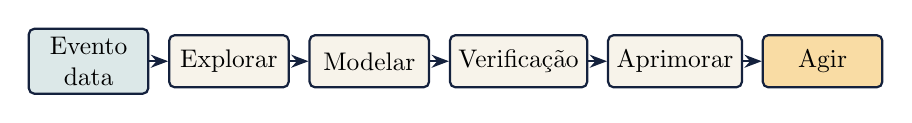
\begin{tikzpicture}[node distance=0.26cm and 0.26cm,scale=0.92,transform shape]
    \node[activity,fill=Mist] (a) {Evento\\data};
    \node[activity,right=of a] (b) {Explorar};
    \node[activity,right=of b] (c) {Modelar};
    \node[activity,right=of c] (d) {Verificação};
    \node[activity,right=of d] (e) {Aprimorar};
    \node[activity,right=of e,fill=Gold!45] (f) {Agir};
    \draw[flow] (a)--(b);
    \draw[flow] (b)--(c);
    \draw[flow] (c)--(d);
    \draw[flow] (d)--(e);
    \draw[flow] (e)--(f);
  \end{tikzpicture}

  \vspace{0.65cm}
  \begin{columns}[T,onlytextwidth]
    \column{0.48\textwidth}
      \textbf{Fundamentos}
      \begin{itemize}
        \item Questões de processo e semântica de eventos
        \item Qualidade de dados e análise exploratória
        \item Modelos comportamentais e descoberta
      \end{itemize}
    \column{0.48\textwidth}
      \textbf{Aplicação}
      \begin{itemize}
        \item Qualidade do modelo e conformidade
        \item Desempenho e perspectivas organizacionais
        \item Análise centrada em objetos e entrega
      \end{itemize}
  \end{columns}
\end{frame}

\begin{frame}{Modelo de funcionamento do curso}
  \begin{columns}[T,onlytextwidth]
    \column{0.52\textwidth}
      \textbf{Cada unidade combina}
      \begin{itemize}
        \item Conceitos e intuição visual
        \item Um exemplo aplicado de log de eventos
        \item Um laboratório com PM4Py
        \item Um breve desafio de interpretação
      \end{itemize}
      \vspace{0.3cm}
      \textbf{Ferramentas principais}\\
      Python, pandas, PM4Py, Jupyter, Graphviz, Git
    \column{0.43\textwidth}
      \begin{block}{Avaliação}
        \begin{tabular}{@{}lr@{}}
          Laboratórios & 30\%\\
          Verificações conceituais & 20\%\\
          Análise do projeto final & 35\%\\
          Apresentação & 15\%
        \end{tabular}
      \end{block}
      \promptbox{Qual processo você encontra toda semana que deixa um rastro digital?}
  \end{columns}
\end{frame}

% ===========================================================================
% Unidade 1
% ===========================================================================
\lecture{Visão Orientada a Processos e Mineração de Processos}{01}
\section{Visão orientada a processos}
\unitdivider{01}{Visão Orientada a Processos e Mineração de Processos}
  {Comece pela questão operacional, não pelo algoritmo.}

\begin{frame}{Um processo é comportamento ao longo do tempo}
  \begin{columns}[T,onlytextwidth]
    \column{0.54\textwidth}
      Um processo é composto por:
      \begin{itemize}
        \item \textbf{casos}: processo instances
        \item \textbf{atividades}: meaningful steps
        \item \textbf{eventos}: recorded atividade executions
        \item \textbf{recursos}: people ou sistemas involved
        \item \textbf{resultados}: tempo, custo, qualidade, compliance
      \end{itemize}
    \column{0.41\textwidth}
      \centering
      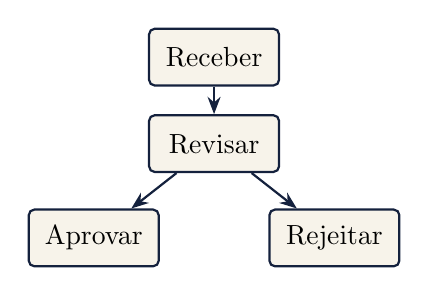
\begin{tikzpicture}[node distance=0.35cm]
        \node[activity] (a) {Receber};
        \node[activity,below=of a] (b) {Revisar};
        \node[activity,below left=0.45cm and -0.15cm of b] (c) {Aprovar};
        \node[activity,below right=0.45cm and -0.15cm of b] (d) {Rejeitar};
        \draw[flow] (a)--(b);
        \draw[flow] (b)--(c);
        \draw[flow] (b)--(d);
      \end{tikzpicture}
  \end{columns}
  \vspace{0.35cm}
  \keyidea{Um modelo de processo é uma afirmação sobre comportamentos possíveis. Um log de eventos é evidência do comportamento observado.}
\end{frame}

\begin{frame}{Quatro perguntas, quatro ramos}
  \centering
  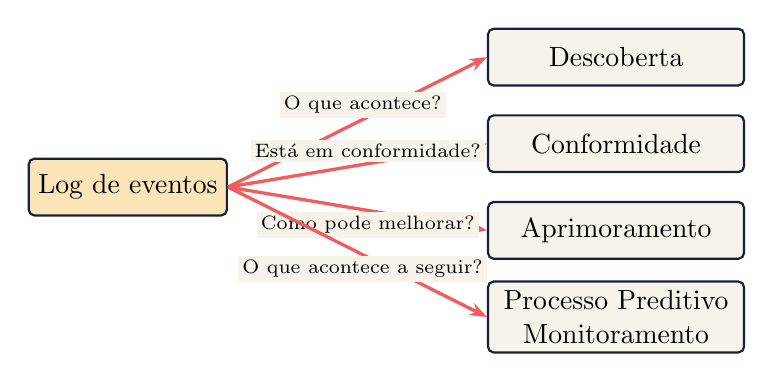
\begin{tikzpicture}[x=1cm,y=1cm]
    \node[activity,fill=Gold!35,minimum width=2.5cm] (log) at (-3.7,0) {Log de eventos};
    \node[activity,minimum width=3.25cm] (disc) at (2.5,1.65) {Descoberta};
    \node[activity,minimum width=3.25cm] (conf) at (2.5,0.55) {Conformidade};
    \node[activity,minimum width=3.25cm] (enh) at (2.5,-0.55) {Aprimoramento};
    \node[activity,minimum width=3.25cm] (pred) at (2.5,-1.65)
      {Processo Preditivo\\Monitoramento};

    \draw[accentflow] (log.east) -- node[pos=0.52,above,fill=Paper,
      inner sep=1.5pt,font=\scriptsize]{O que acontece?} (disc.west);
    \draw[accentflow] (log.east) -- node[pos=0.54,above,fill=Paper,
      inner sep=1.5pt,font=\scriptsize]{Está em conformidade?} (conf.west);
    \draw[accentflow] (log.east) -- node[pos=0.54,below,fill=Paper,
      inner sep=1.5pt,font=\scriptsize]{Como pode melhorar?} (enh.west);
    \draw[accentflow] (log.east) -- node[pos=0.52,below,fill=Paper,
      inner sep=1.5pt,font=\scriptsize]{O que acontece a seguir?} (pred.west);
  \end{tikzpicture}
  \vspace{0.3cm}
  \begin{columns}[T,onlytextwidth]
    \column{0.23\textwidth}\textbf{Descobrir}\\Revele o comportamento real.
    \column{0.23\textwidth}\textbf{Verificação}\\compare o log e o modelo.
    \column{0.23\textwidth}\textbf{Aprimorar}\\Adicione tempo, custo ou decisões.
    \column{0.23\textwidth}\textbf{Prever}\\Antecipe resultados, atrasos e riscos.
  \end{columns}
\end{frame}

\begin{frame}[shrink=5]{Mineração de processos não é um painel}
  \begin{tabular}{@{}>{\bfseries}p{0.20\textwidth}p{0.34\textwidth}p{0.36\textwidth}@{}}
    \toprule
    & Análise tradicional & Mineração de processos\\
    \midrule
    Unidade & Linhas e agregações & Casos e eventos ordenados\\
    Pergunta & Quantos? & Como o trabalho se desenvolveu?\\
    Estrutura & Geralmente tabular & Sequencial, concorrente, cíclico\\
    Saída & KPI ou predição & Comportamento, desvio, desempenho\\
    Risco & Contexto ignorado & Semântica enganosa de caso/evento\\
    \bottomrule
  \end{tabular}
  \vspace{0.5cm}
  \promptbox{Um KPI de entrega piorou. Que perguntas sobre a sequência você faria antes de recomendar uma mudança?}
\end{frame}

\begin{frame}{Estruture uma análise útil}
  \begin{enumerate}
    \item \textbf{decisão}: Que decisão esta análise deve apoiar?
    \item \textbf{Escopo}: Onde o processo começa e termina?
    \item \textbf{Caso}: O que constitui uma instância do processo?
    \item \textbf{Evidência}: Quais sistemas registram os eventos relevantes?
    \item \textbf{Success}: Qual comportamento ou resultado deve mudar?
  \end{enumerate}
  \vspace{0.35cm}
  \begin{block}{Exemplo}
    ``Por que alguns pedidos estão atrasados?'' becomes: ``Quais caminhos, transferências e períodos de espera distinguem os pedidos entregues após a meta de cinco dias?''
  \end{block}
\end{frame}

% ===========================================================================
% Unidade 2
% ===========================================================================
\lecture{Dados de Eventos e Semântica do Log de Eventos}{02}
\section{Semântica do log de eventos}
\unitdivider{02}{Dados de Eventos e Semântica do Log de Eventos}
  {A qualidade da análise começa pelo significado de um evento.}

\begin{frame}{O log de eventos mínimo viável}
  \small
  \begin{tabular}{@{}lllll@{}}
    \toprule
    Caso & Atividade & dados/hora & Recurso & Valor\\
    \midrule
    O-17 & Receber pedido & 09:02 & Portal & 480\\
    O-17 & Verificar crédito & 09:16 & Elena & 480\\
    O-18 & Receber pedido & 09:12 & Portal & 125\\
    O-17 & Aprovar pedido & 10:03 & Marco & 480\\
    O-18 & Verificar crédito & 10:24 & Elena & 125\\
    \bottomrule
  \end{tabular}

  \vspace{0.55cm}
  \begin{columns}[T,onlytextwidth]
    \column{0.31\textwidth}
      \textbf{ID do caso}\\Agrupa eventos relacionados.
    \column{0.31\textwidth}
      \textbf{Atividade}\\Nomeia o que aconteceu.
    \column{0.31\textwidth}
      \textbf{dados/hora}\\Ordena os eventos no tempo.
  \end{columns}
  \vspace{0.35cm}
  \keyidea{Recursos, custos, estados do ciclo de vida e atributos de negócio enriquecem a análise, mas não corrigem uma noção de caso incoerente.}
\end{frame}

\begin{frame}{De eventos a traces e variantes}
  \centering
  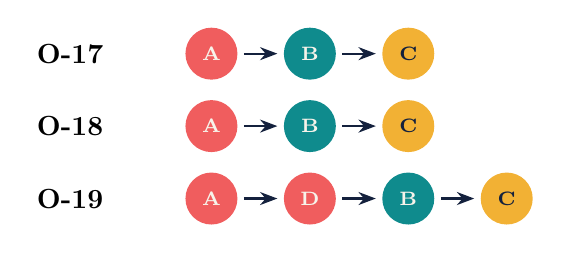
\begin{tikzpicture}[x=1.25cm,y=0.92cm]
    \node[anchor=east,font=\bfseries] at (0,2) {O-17};
    \node[event] at (1,2) {A}; \node[event,fill=Teal] at (2,2) {B};
    \node[event,fill=Gold,text=Ink] at (3,2) {C};
    \draw[flow] (1.33,2)--(1.67,2); \draw[flow] (2.33,2)--(2.67,2);

    \node[anchor=east,font=\bfseries] at (0,1) {O-18};
    \node[event] at (1,1) {A}; \node[event,fill=Teal] at (2,1) {B};
    \node[event,fill=Gold,text=Ink] at (3,1) {C};
    \draw[flow] (1.33,1)--(1.67,1); \draw[flow] (2.33,1)--(2.67,1);

    \node[anchor=east,font=\bfseries] at (0,0) {O-19};
    \node[event] at (1,0) {A}; \node[event,fill=Coral] at (2,0) {D};
    \node[event,fill=Teal] at (3,0) {B}; \node[event,fill=Gold,text=Ink] at (4,0) {C};
    \draw[flow] (1.33,0)--(1.67,0); \draw[flow] (2.33,0)--(2.67,0);
    \draw[flow] (3.33,0)--(3.67,0);
  \end{tikzpicture}

  \vspace{0.35cm}
  \begin{columns}[T,onlytextwidth]
    \column{0.46\textwidth}
      \textbf{Trace}: a sequência ordenada de atividades de um caso.
    \column{0.46\textwidth}
      \textbf{Variante}: um padrão distinto de trace compartilhado por casos.
  \end{columns}
  \vspace{0.25cm}
  Aqui: 3 casos, 2 variantes.
\end{frame}

\begin{frame}{A semântica do ciclo de vida muda a resposta}
  \begin{columns}[T,onlytextwidth]
    \column{0.55\textwidth}
      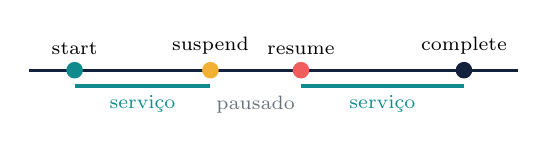
\begin{tikzpicture}[x=1.15cm,y=1cm]
        \draw[very thick,Ink] (0,0)--(5.4,0);
        \foreach \x/\lab/\col in {
          0.5/start/Teal,2.0/suspend/Gold,3.0/resume/Coral,4.8/complete/Ink}
          {
            \fill[\col] (\x,0) circle (3pt);
            \node[above,font=\scriptsize] at (\x,0.08) {\lab};
          }
        \draw[very thick,Teal] (0.5,-0.20)--(2.0,-0.20);
        \draw[very thick,Teal] (3.0,-0.20)--(4.8,-0.20);
        \node[below,font=\scriptsize,text=Teal] at (1.25,-0.2) {serviço};
        \node[below,font=\scriptsize,text=SoftGray] at (2.5,-0.2) {pausado};
        \node[below,font=\scriptsize,text=Teal] at (3.9,-0.2) {serviço};
      \end{tikzpicture}
    \column{0.40\textwidth}
      \textbf{Uma atividade pode emitir vários eventos}
      \begin{itemize}
        \item Iniciar
        \item Suspender / retomar
        \item Concluir
      \end{itemize}
  \end{columns}
  \vspace{0.45cm}
  \keyidea{Sem informações do ciclo de vida, o tempo decorrido pode ser confundido com tempo de trabalho ativo.}
\end{frame}

\begin{frame}[fragile]{Um primeiro log de eventos no PM4Py}
\begin{lstlisting}[style=python]
import pandas as pd
import pm4py

events = pd.read_csv("orders.csv")
events["timestamp"] = pd.to_datetime(
    events["timestamp"], utc=True
)

events = pm4py.format_dataframe(
    events,
    case_id="case_id",
    activity_key="activity",
    timestamp_key="timestamp",
)

pm4py.write_xes(events, "orders.xes")
\end{lstlisting}
  \vspace{0.15cm}
  \textbf{Antes de executar a descoberta:} verifique identificadores, datas/horas, ordenação, duplicatas e o significado dos eventos.
\end{frame}

% ===========================================================================
% Unidade 3
% ===========================================================================
\lecture{Engenharia de Logs de Eventos e Qualidade de Dados}{03}
\section{Engenharia de logs de eventos}
\unitdivider{03}{Engenharia de Logs de Eventos e Qualidade de Dados}
  {Um log de eventos é um artefato analítico projetado, não uma exportação bruta do banco de dados.}

\begin{frame}{Dos sistemas de origem ao log de eventos}
  \centering
  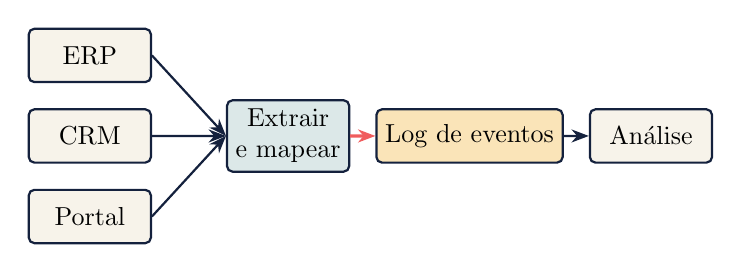
\begin{tikzpicture}[node distance=0.34cm,scale=0.94,transform shape]
    \node[activity] (erp) {ERP};
    \node[activity,below=of erp] (crm) {CRM};
    \node[activity,below=of crm] (web) {Portal};
    \node[activity,right=1.0cm of crm,fill=Mist] (etl) {Extrair\\e mapear};
    \node[activity,right=of etl,fill=Gold!35] (log) {Log de eventos};
    \node[activity,right=of log] (analysis) {Análise};
    \draw[flow] (erp.east)--(etl.west);
    \draw[flow] (crm.east)--(etl.west);
    \draw[flow] (web.east)--(etl.west);
    \draw[accentflow] (etl)--(log);
    \draw[flow] (log)--(analysis);
  \end{tikzpicture}

  \vspace{0.55cm}
  As decisões de mapeamento incluem:
  \begin{itemize}
    \item Qual alteração no banco de dados conta como evento de negócio?
    \item Como os registros são correlacionados em casos?
    \item Quais datas/horas e fusos horários são oficiais?
    \item Quais eventos de baixo nível devem ser abstraídos?
  \end{itemize}
\end{frame}

\begin{frame}{Seis armadilhas comuns de qualidade de dados}
  \begin{columns}[T,onlytextwidth]
    \column{0.47\textwidth}
      \begin{enumerate}
        \item Eventos ausentes
        \item Eventos duplicados
        \item Ordenação incorreta
      \end{enumerate}
    \column{0.47\textwidth}
      \begin{enumerate}
        \setcounter{enumi}{3}
        \item Granularidade mista
        \item Identificadores de caso instáveis
        \item Viés de seleção e extração
      \end{enumerate}
  \end{columns}
  \vspace{0.55cm}
  \begin{block}{Hábito de diagnóstico}
    Para cada padrão surpreendente, pergunte: \textit{Isto é comportamento do processo, do registro ou da extração?}
  \end{block}
\end{frame}

\begin{frame}{O teste da noção de caso}
  Uma noção de caso útil deve responder a três perguntas:
  \begin{enumerate}
    \item Os eventos agrupados pertencem à mesma instância do processo?
    \item A sequência resultante possui início e fim significativos?
    \item Ela apoia a decisão que a análise pretende orientar?
  \end{enumerate}
  \vspace{0.4cm}
  \begin{columns}[T,onlytextwidth]
    \column{0.46\textwidth}
      \begin{block}{Pedido como caso}
        Adequado para lead tempo do cliente e conclusão do pedido.
      \end{block}
    \column{0.46\textwidth}
      \begin{block}{Item como caso}
        Melhor para atendimento parcial e tratamento no nível do item.
      \end{block}
  \end{columns}
\end{frame}

\begin{frame}[shrink=3]{Um relatório compacto de qualidade}
  \small
  \begin{tabular}{@{}p{0.26\textwidth}p{0.26\textwidth}p{0.36\textwidth}@{}}
    \toprule
    Verificação & Evidência & Decisão / limitação\\
    \midrule
    Completude dos casos & 8,4\% não possuem evento final & Excluir casos abertos do KPI de tempo de ciclo\\
    Ordenação temporal & 23 intervalos negativos & Corrigir o desvio conhecido do relógio; sinalizar o restante\\
    Duplicatas & 1,2\% de duplicatas exatas & Remover com uma chave documentada\\
    Significado da atividade & ``Update'' possui 4 fontes & Separar pela semântica de negócio\\
    Cobertura & Os dados começam em jan. de 2025 & Não fazer afirmações sobre versões anteriores do processo\\
    \bottomrule
  \end{tabular}
  \vspace{0.45cm}
  \keyidea{Documentar exclusões faz parte do resultado, não é mera sobrecarga administrativa.}
\end{frame}

\begin{frame}[shrink=8]{Faça o profiling antes de transformar}
  \small
  \begin{tabular}{@{}p{0.19\textwidth}p{0.28\textwidth}p{0.42\textwidth}@{}}
    \toprule
    Nível & Perfil & Decisão que orienta\\
    \midrule
    Evento & Valores ausentes, duplicatas, datas/horas & Corrigir, excluir ou reinterpretar\\
    Caso & Comprimento, duração, completude & Limites e política para casos abertos\\
    Atividade & Frequência, ciclo de vida, recursos & Abstração e filtragem\\
    Variante & Cobertura, raridade, entropia & Estratégia de ruído e segmentação\\
    Temporal & Volume, drift, sazonalidade & Janelas temporais e divisão de avaliação\\
    \bottomrule
  \end{tabular}
  \vspace{0.45cm}
  \keyidea{O profiling não é apenas descritivo. Ele determina quais transformações, modelos e desenhos de avaliação são defensáveis.}
\end{frame}

\begin{frame}[shrink=2]{O flattening é uma escolha de modelagem}
  \begin{columns}[T,onlytextwidth]
    \column{0.54\textwidth}
      \centering
      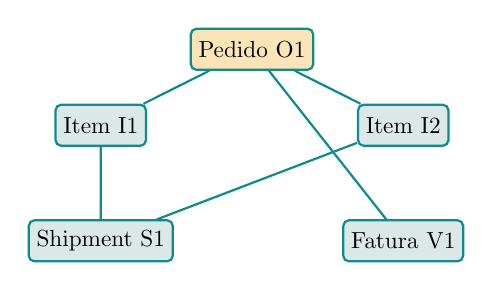
\begin{tikzpicture}[node distance=0.5cm and 0.65cm,scale=0.84,transform shape]
        \node[object,fill=Gold!35] (order) {Pedido O1};
        \node[object,below left=of order] (i1) {Item I1};
        \node[object,below right=of order] (i2) {Item I2};
        \node[object,below=1.1cm of i1] (ship) {Shipment S1};
        \node[object,below=1.1cm of i2] (inv) {Fatura V1};
        \draw[Teal,thick] (order)--(i1);
        \draw[Teal,thick] (order)--(i2);
        \draw[Teal,thick] (i1)--(ship);
        \draw[Teal,thick] (i2)--(ship);
        \draw[Teal,thick] (order)--(inv);
      \end{tikzpicture}
    \column{0.41\textwidth}
      \textbf{Flattening por pedido}
      \begin{itemize}
        \item Eventos compartilhados dos itens convergem
      \end{itemize}
      \textbf{Flattening por item}
      \begin{itemize}
        \item Eventos compartilhados do pedido são duplicados
      \end{itemize}
      \textbf{Manter objetos}
      \begin{itemize}
        \item As relações permanecem explícitas
      \end{itemize}
  \end{columns}
  \vspace{0.35cm}
  \promptbox{Qual noção de caso preserva o comportamento necessário à sua pergunta e quais frequências ela distorce?}
\end{frame}

% ===========================================================================
% Unidade 4
% ===========================================================================
\lecture{Análise Exploratória de Processos}{04}
\section{Análise exploratória}
\unitdivider{04}{Análise Exploratória de Processos}
  {Construa um mapa das evidências antes de construir um modelo de processo.}

\begin{frame}{Explorar em quatro níveis}
  \begin{columns}[T,onlytextwidth]
    \column{0.22\textwidth}
      \begin{block}{Log}
        Casos, eventos, período e cobertura
      \end{block}
    \column{0.22\textwidth}
      \begin{block}{Caso}
        Duração, número de eventos e resultados
      \end{block}
    \column{0.22\textwidth}
      \begin{block}{Atividade}
        Frequência, recursos e temporalidade
      \end{block}
    \column{0.22\textwidth}
      \begin{block}{Variante}
        Caminhos, prevalência, desempenho
      \end{block}
  \end{columns}
  \vspace{0.55cm}
  \promptbox{Qual nível revelaria retrabalho? Qual revelaria uma lacuna sazonal de extração?}
\end{frame}

\begin{frame}{Um grafo diretamente-seguido}
  \centering
  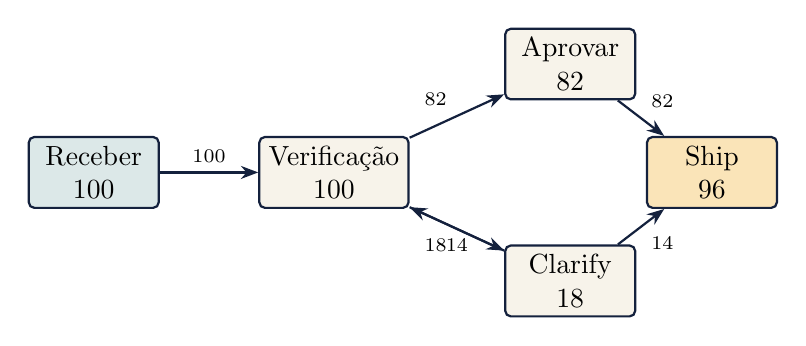
\begin{tikzpicture}[node distance=1.0cm and 1.25cm]
    \node[activity,fill=Mist] (a) {Receber\\100};
    \node[activity,right=of a] (b) {Verificação\\100};
    \node[activity,above right=0.45cm and 1.2cm of b] (c) {Aprovar\\82};
    \node[activity,below right=0.45cm and 1.2cm of b] (d) {Clarify\\18};
    \node[activity,right=3.0cm of b,fill=Gold!35] (e) {Ship\\96};
    \draw[flow] (a)--node[above,font=\scriptsize]{100}(b);
    \draw[flow] (b)--node[above left,font=\scriptsize]{82}(c);
    \draw[flow] (b)--node[below left,font=\scriptsize]{18}(d);
    \draw[flow] (d)--node[below,font=\scriptsize]{14}(b);
    \draw[flow] (c)--node[above right,font=\scriptsize]{82}(e);
    \draw[flow] (d)--node[below right,font=\scriptsize]{14}(e);
  \end{tikzpicture}

  \vspace{0.45cm}
  Um DFG resume a adjacência observada:
  \begin{itemize}
    \item Os nós são atividades; as arestas significam ``diretamente seguido por''
    \item As contagens podem representar frequência ou desempenho
    \item Laços, escolhas e concorrência exigem interpretação cuidadosa
  \end{itemize}
\end{frame}

\begin{frame}{Variantes: úteis, mas fáceis de usar incorretamente}
  \small
  \begin{tabular}{@{}clrr@{}}
    \toprule
    Posição & Variante & casos & Tempo mediano\\
    \midrule
    1 & Receber, Verificação, Aprovar, Ship & 68\% & 2.1 d\\
    2 & Receber, Verificação, Clarify, Verificação, Ship & 14\% & 5.8 d\\
    3 & Receber, Verificação, Rejeitar & 8\% & 1.4 d\\
    4+ & 17 other variants & 10\% & 8.2 d\\
    \bottomrule
  \end{tabular}
  \vspace{0.45cm}
  \begin{columns}[T,onlytextwidth]
    \column{0.47\textwidth}
      \textbf{As variantes revelam}
      \begin{itemize}
        \item Rotas dominantes
        \item Padrões de retrabalho
        \item Comportamento excepcional
      \end{itemize}
    \column{0.47\textwidth}
      \textbf{As variantes podem ocultar}
      \begin{itemize}
        \item Comportamento concorrente
        \item Diferenças de atributos
        \item Casos raros importantes
      \end{itemize}
  \end{columns}
\end{frame}

\begin{frame}[shrink=3]{Uma variante depende da codificação do trace}
  \small
  \begin{tabular}{@{}
    >{\raggedright\arraybackslash}p{0.24\textwidth}
    >{\raggedright\arraybackslash}p{0.36\textwidth}
    >{\raggedright\arraybackslash}p{0.31\textwidth}@{}}
    \toprule
    Codificação & Representação do trace & As variantes distinguem\\
    \midrule
    Fluxo de controle & Sequência de atividades & Diferenças de roteamento\\
    Sensível ao ciclo de vida & Atividade + transição & Início, suspensão, retomada, conclusão\\
    Sensível ao tempo & Atividade + faixa de duração & Regimes comportamentais e temporais\\
    Sensível ao payload & Atividade + atributos selecionados & Coortes de contexto ou resultado\\
    Aprendida & Embedding de sequência/payload & Similaridade além da igualdade exata\\
    \bottomrule
  \end{tabular}
  \vspace{0.4cm}
  \keyidea{As contagens de variantes não são propriedades apenas do log bruto. Elas são produzidas por uma codificação, uma regra de equivalência e um limiar de similaridade.}
\end{frame}

\begin{frame}{Faça o profiling do payload antes de usá-lo}
  \small
  \begin{columns}[T,onlytextwidth]
    \column{0.46\textwidth}
      \begin{block}{Payload do evento}
        Informação transportada por um evento além do caso, da atividade e da dados/hora.
      \end{block}
      \begin{itemize}
        \item Atributos estruturados e medições
        \item Texto, documentos, imagens, áudio e referências de sensores
        \item Contexto de recurso, custo, localização e produto
      \end{itemize}
    \column{0.46\textwidth}
      \textbf{Faça o profiling antes da codificação}
      \begin{itemize}
        \item Disponibilidade no momento do evento
        \item Valores ausentes e cardinalidade
        \item Drift, semântica e cardinalidade
        \item Privacidade, proxies e vazamento de informação futura
      \end{itemize}
  \end{columns}
  \vspace{0.05cm}
  \promptbox{Use dimensões do payload somente quando servirem à pergunta analítica; caso contrário, podem fragmentar traces em variantes sem significado com apenas um caso.}
\end{frame}

\begin{frame}{Fronteira de Pareto para detecção de variantes}
  \scriptsize
  \begin{columns}[T,onlytextwidth]
    \column{0.56\textwidth}
      \centering
      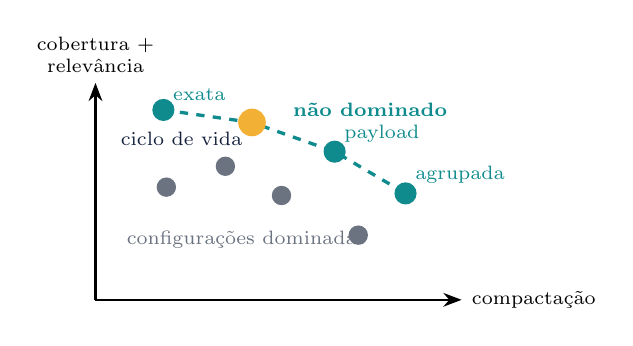
\begin{tikzpicture}[x=0.75cm,y=0.53cm]
        \draw[-{Stealth},thick] (0,0)--(6.2,0)
          node[right,font=\scriptsize]{compactação};
        \draw[-{Stealth},thick] (0,0)--(0,5.2)
          node[above,font=\scriptsize,align=center]{cobertura +\\relevância};

        \draw[Teal,very thick,dashed]
          (1.15,4.55)--(2.65,4.25)--(4.05,3.55)--(5.25,2.55);
        \fill[Teal] (1.15,4.55) circle (4pt)
          node[above right,font=\scriptsize]{exata};
        \fill[Gold] (2.65,4.25) circle (5pt)
          node[below left,font=\scriptsize,text=Ink]{ciclo de vida};
        \fill[Teal] (4.05,3.55) circle (4pt)
          node[above right,font=\scriptsize]{payload};
        \fill[Teal] (5.25,2.55) circle (4pt)
          node[above right,font=\scriptsize]{agrupada};

        \foreach \x/\y in {1.2/2.7,2.2/3.2,3.15/2.5,4.45/1.55}
          \fill[SoftGray] (\x,\y) circle (3.5pt);
        \node[Teal,font=\scriptsize\bfseries] at (4.65,4.55)
          {não dominado};
        \node[SoftGray,font=\scriptsize] at (2.55,1.45)
          {configurações dominadas};
      \end{tikzpicture}
    \column{0.39\textwidth}
      \textbf{Configurações candidatas}\\
      Codificação, limiar de similaridade, corte de variantes raras e dimensões do payload.

      \vspace{0.25cm}
      \textbf{Objetivos}\\
      Cobertura de casos, compactação, relevância para a decisão e estabilidade temporal.
  \end{columns}
  \vspace{0.1cm}
  \centering\textbf{\color{Teal}Inspecione traces representativos antes de selecionar uma configuração não dominada.}
\end{frame}

\begin{frame}[shrink=4]{Um perfil de prontidão para modelagem}
  Antes da descoberta ou predição, registre:
  \begin{columns}[T,onlytextwidth]
    \column{0.47\textwidth}
      \begin{itemize}
        \item Distribuições de casos e comprimentos de traces
        \item Cobertura de variantes e comportamento de cauda longa
        \item Desbalanceamento de classes e resultados
        \item Atributos ausentes e de alta cardinalidade
      \end{itemize}
    \column{0.47\textwidth}
      \begin{itemize}
        \item Drift do processo e da população
        \item Casos abertos versus concluídos
        \item Datas/horas de observação e do rótulo
        \item Possível vazamento de informação futura
      \end{itemize}
  \end{columns}
  \vspace{0.4cm}
  \begin{block}{Entrega}
    Um relatório de prontidão de uma página: população utilizável, distorções conhecidas, escolha de representação, estratégia de divisão e informações excluídas.
  \end{block}
\end{frame}

\begin{frame}[fragile]{Exploração com PM4Py}
\begin{lstlisting}[style=python]
import pm4py

print(pm4py.get_start_activities(log))
print(pm4py.get_end_activities(log))

variants = pm4py.get_variants_as_tuples(log)
dfg, starts, ends = pm4py.discover_dfg(log)

filtered = pm4py.filter_case_performance(
    log,
    min_performance=5 * 24 * 60 * 60,
)
\end{lstlisting}
  \vspace{0.15cm}
  \textbf{Tarefa de interpretação:} compare casos comuns com casos lentos. Quais diferenças de caminho são explicações plausíveis e quais exigem mais evidências?
\end{frame}

% ===========================================================================
% Unidade 5
% ===========================================================================
\lecture{Fundamentos de Modelagem de Processos}{05}
\section{Fundamentos de modelagem}
\unitdivider{05}{Fundamentos de Modelagem de Processos}
  {Representações diferentes respondem a perguntas diferentes.}

\begin{frame}{Quatro blocos fundamentais de comportamento}
  \begin{columns}[T,onlytextwidth]
    \column{0.22\textwidth}
      \begin{block}{Sequência}
        $A \rightarrow B$
      \end{block}
      Uma segue a outra.
    \column{0.22\textwidth}
      \begin{block}{Escolha}
        $A \rightarrow (B|C)$
      \end{block}
      Um ramo é selecionado.
    \column{0.22\textwidth}
      \begin{block}{Paralelo}
        $A \rightarrow (B \parallel C)$
      \end{block}
      Ambas ocorrem; a ordem varia.
    \column{0.22\textwidth}
      \begin{block}{Laço}
        $A \rightarrow B \rightarrow A$
      \end{block}
      O comportamento se repete.
  \end{columns}
  \vspace{0.55cm}
  \keyidea{Um modelo útil deve distinguir escolha de concorrência e permitir repetição sem permitir tudo.}
\end{frame}

\begin{frame}{Um DFG não é um modelo de processo completo}
  \begin{columns}[T,onlytextwidth]
    \column{0.48\textwidth}
      \centering
      \textbf{Traces observados}\\[0.25cm]
      $\langle A,B,C,D\rangle$\\
      $\langle A,C,B,D\rangle$\\[0.45cm]
      As evidências sugerem que $B$ e $C$ podem ocorrer em paralelo.
    \column{0.48\textwidth}
      \centering
      \textbf{DFG}\\[0.2cm]
      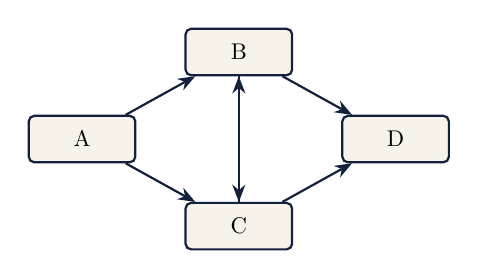
\begin{tikzpicture}[node distance=0.6cm and 0.75cm,scale=0.82,transform shape]
        \node[activity] (a) {A};
        \node[activity,above right=of a] (b) {B};
        \node[activity,below right=of a] (c) {C};
        \node[activity,below right=of b] (d) {D};
        \draw[flow] (a)--(b); \draw[flow] (a)--(c);
        \draw[flow] (b)--(c); \draw[flow] (c)--(b);
        \draw[flow] (b)--(d); \draw[flow] (c)--(d);
      \end{tikzpicture}
  \end{columns}
  \vspace{0.55cm}
  O DFG também parece permitir alternância repetida entre $B$ e $C$.
  Esse comportamento nunca foi observado.
\end{frame}

\begin{frame}{Representações de modelos}
  \small
  \begin{tabular}{@{}p{0.20\textwidth}p{0.30\textwidth}p{0.40\textwidth}@{}}
    \toprule
    Representação & Ponto forte & Atenção a\\
    \midrule
    DFG & Visão geral rápida e legível & Sem semântica completa de execução\\
    Árvore de processos & Estruturada e sound por construção & Restringe a forma do modelo\\
    Rede de Petri & Concorrência e replay precisos & Mais difícil para não especialistas\\
    BPMN & Notação de negócio familiar & A semântica varia conforme o uso\\
    Transition sistema & Comportamento baseado em estados & Explosão de estados\\
    \bottomrule
  \end{tabular}
  \vspace{0.5cm}
  \promptbox{Qual representação você usaria para discutir com stakeholders? E para verificação de conformidade baseada em alinhamentos?}
\end{frame}

\begin{frame}[shrink=4]{Escolha uma estratégia de modelagem}
  \small
  \begin{tabular}{@{}
    >{\raggedright\arraybackslash}p{0.19\textwidth}
    >{\raggedright\arraybackslash}p{0.23\textwidth}
    >{\raggedright\arraybackslash}p{0.24\textwidth}
    >{\raggedright\arraybackslash}p{0.24\textwidth}@{}}
    \toprule
    Finalidade & Estratégia & Representação & Ênfase\\
    \midrule
    Explicar o fluxo & Descoberta estruturada & Árvore de processos / BPMN & Simplicidade, fitness\\
    Auditar regras & Modelagem normativa & Rede de Petri / Declare & Soundness, diagnósticos\\
    Explorar a complexidade & Descoberta sensível à frequência & DFG / rede heurística & Cobertura, legibilidade\\
    Prever o estado & Modelo de estado ou prefixo & Transição/features & Generalização, utilidade\\
    Comunicar & Simplificar e anotar & BPMN / DFG & Interpretabilidade\\
    \bottomrule
  \end{tabular}
  \vspace{0.45cm}
  \keyidea{Não existe ``melhor modelo independente do contexto.'' Declare a finalidade antes de selecionar o algoritmo, a representação e os critérios de qualidade.}
\end{frame}

\begin{frame}{Abstração antes do algoritmo}
  \centering
  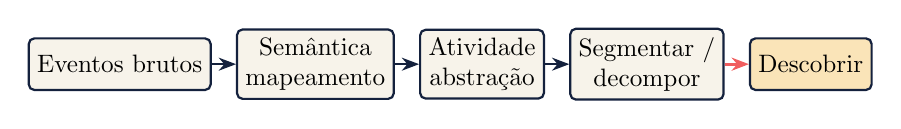
\begin{tikzpicture}[node distance=0.34cm,scale=0.91,transform shape]
    \node[activity] (raw) {Eventos brutos};
    \node[activity,right=of raw] (semantic) {Semântica\\mapeamento};
    \node[activity,right=of semantic] (abstract) {Atividade\\abstração};
    \node[activity,right=of abstract] (segment) {Segmentar /\\decompor};
    \node[activity,right=of segment,fill=Gold!35] (discover) {Descobrir};
    \draw[flow] (raw)--(semantic);
    \draw[flow] (semantic)--(abstract);
    \draw[flow] (abstract)--(segment);
    \draw[accentflow] (segment)--(discover);
  \end{tikzpicture}
  \vspace{0.55cm}
  \begin{columns}[T,onlytextwidth]
    \column{0.47\textwidth}
      \textbf{Estratégias úteis}
      \begin{itemize}
        \item Agrupar eventos técnicos
        \item Separar populações do processo
        \item Decompor por ciclo de vida ou subprocesso
      \end{itemize}
    \column{0.47\textwidth}
      \textbf{Prática}
      \begin{itemize}
        \item Versionar cada mapeamento
        \item Comparar perfis antes e depois
        \item Manter um vínculo rastreável com o evento bruto
      \end{itemize}
  \end{columns}
\end{frame}

\begin{frame}{Soundness: todo caso pode terminar corretamente?}
  Para um modelo de fluxo de trabalho, geralmente desejamos:
  \begin{itemize}
    \item Um início e uma conclusão significativos
    \item Toda atividade modelada pode ocorrer
    \item Nenhum deadlock antes da conclusão
    \item Nenhum token ou trabalho residual após a conclusão
  \end{itemize}
  \vspace{0.35cm}
  \begin{block}{Por que isso importa}
    Um diagrama atraente ainda pode codificar comportamentos impossíveis ou incompletos.
    A semântica formal permite testar o modelo em vez de confiar em sua aparência.
  \end{block}
\end{frame}

% ===========================================================================
% Unidade 6
% ===========================================================================
\lecture{Descoberta de Processos}{06}
\section{Descoberta de processos}
\unitdivider{06}{Descoberta de Processos}
  {Algoritmos de descoberta condensam o comportamento dos eventos em um modelo explicativo.}

\begin{frame}{A descoberta exige equilíbrio}
  \centering
  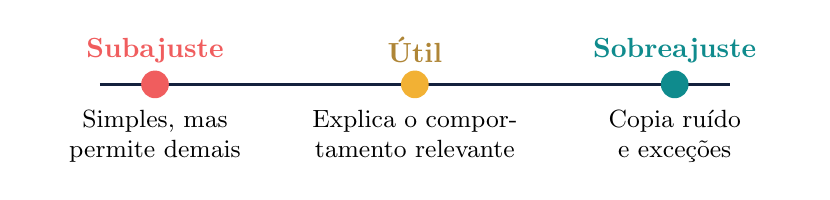
\begin{tikzpicture}
    \draw[very thick,Ink] (-4,0)--(4,0);
    \fill[Coral] (-3.3,0) circle (5pt);
    \fill[Gold] (0,0) circle (5pt);
    \fill[Teal] (3.3,0) circle (5pt);
    \node[above,text=Coral,font=\bfseries] at (-3.3,0.15) {Subajuste};
    \node[above,text=Gold!70!Ink,font=\bfseries] at (0,0.15) {Útil};
    \node[above,text=Teal,font=\bfseries] at (3.3,0.15) {Sobreajuste};
    \node[below,text width=3cm,align=center,font=\small] at (-3.3,-0.2)
      {Simples, mas permite demais};
    \node[below,text width=3cm,align=center,font=\small] at (0,-0.2)
      {Explica o comportamento relevante};
    \node[below,text width=3cm,align=center,font=\small] at (3.3,-0.2)
      {Copia ruído e exceções};
  \end{tikzpicture}
  \vspace{0.8cm}
  A descoberta depende de:
  \begin{itemize}
    \item O log de eventos e seu nível de abstração
    \item As premissas comportamentais do algoritmo
    \item Limiares de ruído e frequência
    \item O uso pretendido do modelo resultante
  \end{itemize}
\end{frame}

\begin{frame}{Três famílias de descoberta}
  \begin{columns}[T,onlytextwidth]
    \column{0.30\textwidth}
      \begin{block}{Alpha Miner}
        Usa relações de ordenação para inferir comportamentos causais, paralelos e de escolha.
      \end{block}
      Mais indicado como fundamento conceitual.
    \column{0.30\textwidth}
      \begin{block}{Heuristics Miner}
        Usa medidas de frequência e dependência para tolerar ruído.
      \end{block}
      Útil para modelos exploratórios.
    \column{0.30\textwidth}
      \begin{block}{Inductive Miner}
        Encontra recursivamente cortes de sequência, escolha, paralelismo e laço.
      \end{block}
      Produz modelos estruturados e sound.
  \end{columns}
\end{frame}

\begin{frame}{Um experimento disciplinado de descoberta}
  \centering
  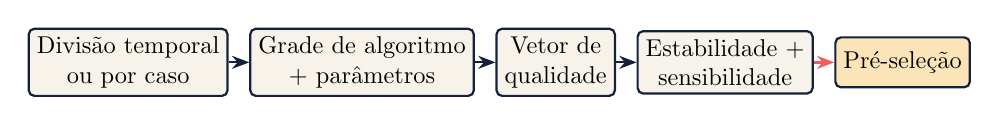
\begin{tikzpicture}[node distance=0.30cm,scale=0.88,transform shape]
    \node[activity] (split) {Divisão temporal\\ou por caso};
    \node[activity,right=of split] (grid) {Grade de algoritmo\\+ parâmetros};
    \node[activity,right=of grid] (quality) {Vetor de\\qualidade};
    \node[activity,right=of quality] (stable) {Estabilidade +\\sensibilidade};
    \node[activity,right=of stable,fill=Gold!35] (short) {Pré-seleção};
    \draw[flow] (split)--(grid);
    \draw[flow] (grid)--(quality);
    \draw[flow] (quality)--(stable);
    \draw[accentflow] (stable)--(short);
  \end{tikzpicture}
  \vspace{0.55cm}
  \begin{enumerate}
    \item Defina restrições e direções das métricas antes de ver os resultados.
    \item Mantenha os dados de descoberta separados dos dados de avaliação final.
    \item Mantenha todos os parâmetros e artefatos candidatos, não apenas o vencedor.
    \item Inspecione atividades e arestas instáveis, não apenas pontuações agregadas.
  \end{enumerate}
\end{frame}

\begin{frame}{Intuição da descoberta indutiva}
  \centering
  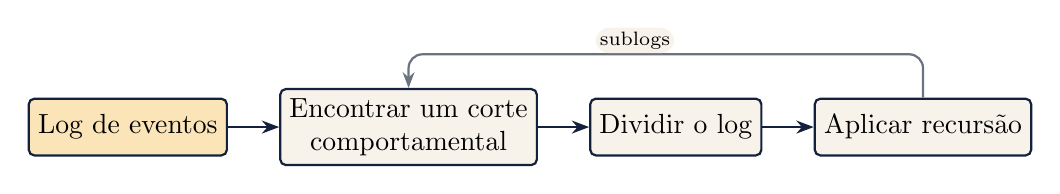
\begin{tikzpicture}[node distance=0.45cm and 0.65cm]
    \node[activity,fill=Gold!35] (log) {Log de eventos};
    \node[activity,right=of log] (cut) {Encontrar um corte\\comportamental};
    \node[activity,right=of cut] (split) {Dividir o log};
    \node[activity,right=of split] (rec) {Aplicar recursão};
    \draw[flow] (log)--(cut);
    \draw[flow] (cut)--(split);
    \draw[flow] (split)--(rec);
    \draw[softflow,rounded corners=5pt]
      (rec.north) -- ++(0,0.55)
      -| node[pos=0.28,above,font=\scriptsize,fill=Paper,inner sep=1.5pt]
        {sublogs}
      (cut.north);
  \end{tikzpicture}
  \vspace{0.55cm}
  Cortes candidatos:
  \begin{columns}[T,onlytextwidth]
    \column{0.22\textwidth}\centering Sequência\\$\rightarrow$
    \column{0.22\textwidth}\centering Escolha exclusiva\\$\times$
    \column{0.22\textwidth}\centering Paralelo\\$\wedge$
    \column{0.22\textwidth}\centering Laço\\$\circlearrowleft$
  \end{columns}
  \vspace{0.45cm}
  \keyidea{O resultado é uma árvore de processos que pode ser traduzida em uma rede de Petri ou modelo BPMN.}
\end{frame}

\begin{frame}[fragile]{Descoberta com PM4Py}
\begin{lstlisting}[style=python]
import pm4py

# Structured discovery
tree = pm4py.discover_process_tree_inductive(
    log, noise_threshold=0.2
)
net, initial, final = pm4py.convert_to_petri_net(tree)

# Business-facing representation
bpmn = pm4py.convert_to_bpmn(tree)
pm4py.save_vis_bpmn(bpmn, "discovered_process.svg")
\end{lstlisting}
  \vspace{0.15cm}
  \textbf{Experimento:} varie o limiar de ruído. Registre quais comportamentos desaparecem, quais permanecem e se o modelo se torna mais útil.
\end{frame}

% ===========================================================================
% Unidade 7
% ===========================================================================
\lecture{Qualidade e Avaliação de Modelos}{07}
\section{Qualidade do modelo}
\unitdivider{07}{Qualidade e Avaliação de Modelos}
  {Nenhuma pontuação isolada informa se um modelo é adequado à sua finalidade.}

\begin{frame}{As quatro dimensões de qualidade}
  \begin{columns}[T,onlytextwidth]
    \column{0.22\textwidth}
      \begin{block}{Fitness}
        O modelo consegue reproduzir o comportamento observado?
      \end{block}
    \column{0.22\textwidth}
      \begin{block}{Precisão}
        Ele evita permitir comportamentos não observados?
      \end{block}
    \column{0.22\textwidth}
      \begin{block}{Generalização}
        Ele lida com comportamentos futuros plausíveis?
      \end{block}
    \column{0.22\textwidth}
      \begin{block}{Simplicidade}
        As pessoas conseguem compreendê-lo e utilizá-lo?
      \end{block}
  \end{columns}
  \vspace{0.55cm}
  \keyidea{Fitness perfeito é trivial se o modelo permite todo trace possível.
  A qualidade emerge do compromisso entre as dimensões.}
\end{frame}

\begin{frame}{Construa um vetor de qualidade, não uma única pontuação}
  \scriptsize
  \begin{tabular}{@{}p{0.20\textwidth}p{0.32\textwidth}p{0.36\textwidth}@{}}
    \toprule
    Dimensão & Exemplo de medida & Risco de interpretação\\
    \midrule
    Fitness & Fitness por alinhamento/replay & Favorece modelos permissivos\\
    Precisão & Precisão por escaping edges/alinhamento & Sensível à cobertura do log\\
    Generalização & Replay em holdout, validação cruzada & Depende do desenho da divisão\\
    Simplicidade & Nós, arcos e complexidade do fluxo de controle & Pequeno nem sempre é compreensível\\
    Estabilidade & Frequência de arestas/relações por bootstrap & Pontuações agregadas podem ocultar instabilidade\\
    Viabilidade & Soundness, tempo de execução, memória & Restrições rígidas, não preferências\\
    \bottomrule
  \end{tabular}
  \vspace{0.2cm}
  \keyidea{Registre a direção da métrica, o método de cálculo, a divisão dos dados e a incerteza de cada componente do vetor de qualidade.}
\end{frame}

\begin{frame}{Fitness e precisão atuam em direções opostas}
  \centering
  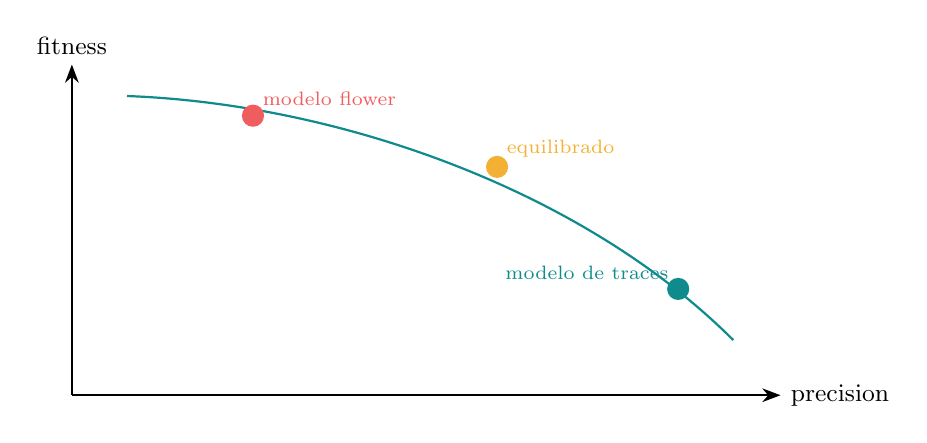
\begin{tikzpicture}[x=1cm,y=1cm]
    \draw[-{Stealth},thick] (0,0)--(9,0) node[right,font=\small]{precision};
    \draw[-{Stealth},thick] (0,0)--(0,4.2) node[above,font=\small]{fitness};
    \draw[thick,Teal] (0.7,3.8) .. controls (3.4,3.7) and (6.5,2.6) .. (8.4,0.7);
    \fill[Coral] (2.3,3.55) circle (4pt) node[above right,font=\scriptsize]{modelo flower};
    \fill[Gold] (5.4,2.9) circle (4pt) node[above right,font=\scriptsize]{equilibrado};
    \fill[Teal] (7.7,1.35) circle (4pt) node[above left,font=\scriptsize]{modelo de traces};
  \end{tikzpicture}
  \par
  \vspace{0.25cm}
  O ponto ``melhor'' depende de o modelo servir à explicação, simulação, conformidade ou predição.
\end{frame}

\begin{frame}{Por que uma média ponderada pode enganar}
  Suponha:
  \[
    score = 0.4\,fitness + 0.4\,precision + 0.2\,simplicidade
  \]
  \begin{columns}[T,onlytextwidth]
    \column{0.47\textwidth}
      \textbf{O que isso oculta}
      \begin{itemize}
        \item Um mínimo crítico pode ser violado
        \item Pesos diferentes invertem o ranking
        \item Compensar métricas pode ser inaceitável
        \item Escala e normalização alteram o resultado
      \end{itemize}
    \column{0.47\textwidth}
      \textbf{Primeiro passo melhor}
      \begin{itemize}
        \item Aplicar restrições rígidas de viabilidade
        \item Remover candidatos dominados
        \item Inspecionar a fronteira de Pareto
        \item Adicionar preferências somente depois
      \end{itemize}
  \end{columns}
\end{frame}

\begin{frame}{Dominância e fronteira de Pareto}
  \begin{columns}[T,onlytextwidth]
    \column{0.57\textwidth}
      \centering
      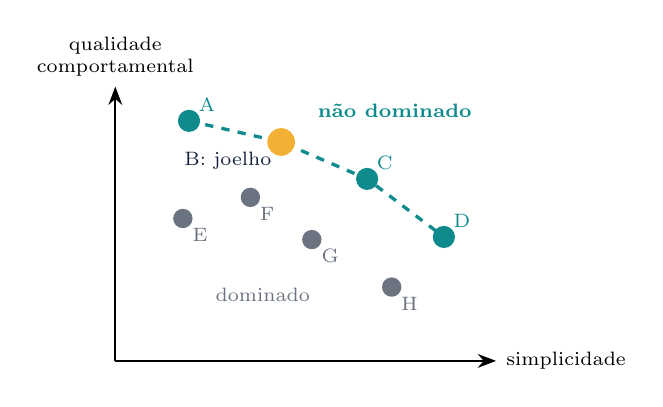
\begin{tikzpicture}[x=0.78cm,y=0.67cm]
        \draw[-{Stealth},thick] (0,0)--(6.2,0)
          node[right,font=\scriptsize]{simplicidade};
        \draw[-{Stealth},thick] (0,0)--(0,5.2)
          node[above,font=\scriptsize,align=center]{qualidade\\comportamental};

        \draw[Teal,very thick,dashed]
          (1.2,4.55)--(2.7,4.15)--(4.1,3.45)--(5.35,2.35);
        \foreach \x/\y/\lab in {
          1.2/4.55/A,4.1/3.45/C,5.35/2.35/D}
          \fill[Teal] (\x,\y) circle (4pt)
            node[above right,font=\scriptsize]{\lab};
        \fill[Gold] (2.7,4.15) circle (5pt)
          node[below left,font=\scriptsize,text=Ink]{B: joelho};

        \foreach \x/\y/\lab in {
          1.1/2.7/E,2.2/3.1/F,3.2/2.3/G,4.5/1.4/H}
          \fill[SoftGray] (\x,\y) circle (3.5pt)
            node[below right,font=\scriptsize]{\lab};
        \node[Teal,font=\scriptsize\bfseries] at (4.55,4.75)
          {não dominado};
        \node[SoftGray,font=\scriptsize] at (2.4,1.25)
          {dominado};
      \end{tikzpicture}
    \column{0.38\textwidth}
      O candidato $X$ domina $Y$ quando:
      \begin{itemize}
        \item $X$ não é pior em nenhum objetivo
        \item $X$ é melhor em pelo menos um objetivo
      \end{itemize}
      \vspace{0.1cm}
      A \textbf{fronteira de Pareto} contém candidatos que não são dominados por nenhum outro.
  \end{columns}
  \vspace{0.05cm}
  \keyidea{Um ponto de joelho oferece um bom compromisso, mas é candidato à discussão, não um vencedor automático.}
\end{frame}

\begin{frame}{Seleção prática na fronteira de Pareto}
  \begin{enumerate}
    \item \textbf{Primeiro, imponha restrições}: exija soundness, fitness mínimo e tempo de execução ou tamanho do modelo aceitável.
    \item \textbf{Estime a incerteza}: faça bootstrap dos casos ou repita folds temporais; não confie em diferenças mínimas de pontuação.
    \item \textbf{Inspecione a sensibilidade}: varie limiares, abstração de atividades e implementação das métricas.
    \item \textbf{Revise a fronteira}: mostre todos os modelos não dominados e explique o que se ganha e perde entre candidatos adjacentes.
    \item \textbf{Selecione com transparência}: use um ponto de joelho, regra lexicográfica ou utilidade dos stakeholders após conhecer a fronteira.
    \item \textbf{Valide uma vez}: reporte a escolha final em dados holdout intocados.
  \end{enumerate}
\end{frame}

\begin{frame}{Replay e alinhamentos}
  \begin{columns}[T,onlytextwidth]
    \column{0.47\textwidth}
      \begin{block}{Replay baseado em tokens}
        Reproduz traces em uma rede de Petri e conta tokens ausentes, restantes, consumidos e produzidos.
      \end{block}
      Rápido e diagnóstico, mas pode mascarar alguns desvios.
    \column{0.47\textwidth}
      \begin{block}{Alinhamentos}
        Encontra uma correspondência de custo mínimo entre o comportamento do log e o modelo.
      \end{block}
      Mais preciso, porém computacionalmente mais caro.
  \end{columns}
  \vspace{0.55cm}
  \promptbox{Você avaliaria um modelo de conformidade e um modelo exploratório com a mesma tolerância a desvios? Por quê?}
\end{frame}

\begin{frame}[fragile]{Avalie os candidatos}
\begin{lstlisting}[style=python]
fitness = pm4py.fitness_alignments(
    log, net, initial, final
)
precision = pm4py.precision_alignments(
    log, net, initial, final
)

print(fitness["log_fitness"])
print(precision)
\end{lstlisting}
  \vspace{0.2cm}
  Uma comparação defensável registra:
  \begin{itemize}
    \item Pontuações e tempo de execução
    \item Tamanho e legibilidade do modelo
    \item Desempenho em treinamento versus holdout
    \item Qual comportamento importa para a pergunta analítica
  \end{itemize}
\end{frame}

\begin{frame}{Um protocolo de avaliação defensável}
  \centering
  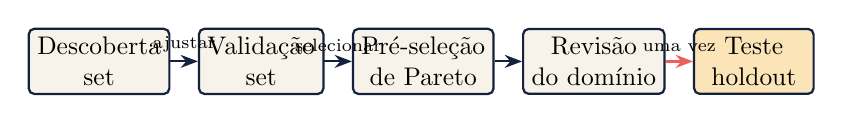
\begin{tikzpicture}[node distance=0.38cm,scale=0.92,transform shape]
    \node[activity] (train) {Descoberta\\set};
    \node[activity,right=of train] (valid) {Validação\\set};
    \node[activity,right=of valid] (pareto) {Pré-seleção\\de Pareto};
    \node[activity,right=of pareto] (review) {Revisão\\do domínio};
    \node[activity,right=of review,fill=Gold!35] (test) {Teste\\holdout};
    \draw[flow] (train)--node[above,font=\scriptsize]{ajustar}(valid);
    \draw[flow] (valid)--node[above,font=\scriptsize]{selecionar}(pareto);
    \draw[flow] (pareto)--(review);
    \draw[accentflow] (review)--node[above,font=\scriptsize]{uma vez}(test);
  \end{tikzpicture}
  \vspace{0.55cm}
  relatório:
  \begin{itemize}
    \item Regras de geração e candidatos excluídos
    \item Vetores completos de métricas com incerteza, não apenas o modelo selecionado
    \item Pertencimento à fronteira de Pareto e regra de decisão final
    \item Desempenho em holdout, instabilidade conhecida e uso pretendido do modelo
  \end{itemize}
\end{frame}

% ===========================================================================
% Unidade 8
% ===========================================================================
\lecture{Verificação de Conformidade}{08}
\section{Verificação de conformidade}
\unitdivider{08}{Verificação de Conformidade}
  {Encontre a menor explicação significativa de como a realidade e o modelo diferem.}

\begin{frame}{O que conta como não conformidade?}
  \begin{columns}[T,onlytextwidth]
    \column{0.46\textwidth}
      \textbf{O modelo pode ser normativo}
      \begin{itemize}
        \item Política
        \item Regulação
        \item Procedimento operacional padrão
      \end{itemize}
      Um desvio pode indicar risco.
    \column{0.46\textwidth}
      \textbf{O modelo pode ser descritivo}
      \begin{itemize}
        \item Descoberta anterior
        \item Padrão operacional esperado
        \item Baseline de simulação
      \end{itemize}
      Um desvio pode indicar mudança.
  \end{columns}
  \vspace{0.5cm}
  \keyidea{A conformidade identifica diferenças. O contexto do domínio determina se elas são prejudiciais, úteis ou apenas ausentes do modelo.}
\end{frame}

\begin{frame}{Lendo um alinhamento}
  \small
  \begin{tabular}{@{}lccccc@{}}
    \toprule
    Posição & 1 & 2 & 3 & 4 & 5\\
    \midrule
    Log & Receber & Verificação & Clarify & Aprovar & Ship\\
    Modelar & Receber & Verificação & $\gg$ & Aprovar & Ship\\
    Movimento & síncrono & síncrono & log & síncrono & síncrono\\
    \bottomrule
  \end{tabular}
  \vspace{0.55cm}
  \begin{columns}[T,onlytextwidth]
    \column{0.30\textwidth}
      \textbf{Movimento síncrono}\\Evento e modelo concordam.
    \column{0.30\textwidth}
      \textbf{Movimento no log}\\Evento observado sem correspondência.
    \column{0.30\textwidth}
      \textbf{Movimento no modelo}\\Comportamento esperado não observado.
  \end{columns}
\end{frame}

\begin{frame}{Dos desvios aos achados}
  \begin{enumerate}
    \item \textbf{Localize}: Quais atividades, caminhos e casos apresentam desvios?
    \item \textbf{Quantifique}: Quão frequentes, custosos ou atrasados são?
    \item \textbf{Segmente}: Quais produtos, equipes ou períodos diferem?
    \item \textbf{Validar}: O modelo está atualizado e os dados estão completos?
    \item \textbf{Explicar}: Qual mecanismo operacional poderia produzir isso?
  \end{enumerate}
  \vspace{0.4cm}
  \begin{block}{Achado sólido}
    ``A revisão manual de crédito é ignorada em 7,3\% dos pedidos de alto valor, concentrados em um canal após a versão de abril do sistema.''
  \end{block}
\end{frame}

\begin{frame}[fragile]{Diagnósticos de alinhamento no PM4Py}
\begin{lstlisting}[style=python]
alignments = pm4py.conformance_diagnostics_alignments(
    log, net, initial, final
)

for result in alignments[:3]:
    print(result["fitness"])
    print(result["alignment"])
\end{lstlisting}
  \vspace{0.15cm}
  \textbf{Saída do laboratório:} uma tabela ordenada de desvios contendo padrão, casos afetados, frequência, impacto no desempenho e interpretação validada.
\end{frame}

% ===========================================================================
% Unidade 9
% ===========================================================================
\lecture{Desempenho e Aprimoramento de Processos}{09}
\section{Aprimoramento de processos}
\unitdivider{09}{Desempenho e Aprimoramento de Processos}
  {Um gargalo é um mecanismo, não apenas um número vermelho.}

\begin{frame}{Decomponha o tempo decorrido}
  \centering
  
\begin{tikzpicture}[x=1.25cm,y=1cm]
    \draw[very thick,Ink] (0,0)--(8,0);
    \fill[Teal] (0.4,0) circle (4pt);
    \fill[Coral] (2.6,0) circle (4pt);
    \fill[Teal] (4.0,0) circle (4pt);
    \fill[Coral] (7.5,0) circle (4pt);
    \draw[line width=6pt,Teal] (0.4,-0.22)--(1.2,-0.22);
    \draw[line width=6pt,Mist] (1.2,-0.22)--(2.6,-0.22);
    \draw[line width=6pt,Teal] (2.6,-0.22)--(4.0,-0.22);
    \draw[line width=6pt,Mist] (4.0,-0.22)--(7.5,-0.22);
    \node[below,font=\scriptsize] at (0.8,-0.3) {serviço};
    \node[below,font=\scriptsize] at (1.9,-0.3) {waiting};
    \node[below,font=\scriptsize] at (3.3,-0.3) {serviço};
    \node[below,font=\scriptsize] at (5.75,-0.3) {waiting};
  \end{tikzpicture}
  \vspace{0.55cm}
  \begin{columns}[T,onlytextwidth]
    \column{0.30\textwidth}\textbf{Tempo total de atravessamento}\\Do início à conclusão do caso.
    \column{0.30\textwidth}\textbf{Tempo de serviço}\\Tempo de trabalho ativo.
    \column{0.30\textwidth}\textbf{Tempo de espera}\\Tempo entre atividades.
  \end{columns}
\end{frame}

\begin{frame}{Quatro sinais de gargalo}
  \begin{columns}[T,onlytextwidth]
    \column{0.47\textwidth}
      \begin{itemize}
        \item Longa espera antes de uma atividade
        \item Fila crescente ao longo do tempo
        \item Retrabalho retornando à mesma atividade
        \item Excesso de transferências antes da conclusão
      \end{itemize}
    \column{0.47\textwidth}
      \begin{block}{Não pare em}
        ``A atividade X possui a maior duração média.''
      \end{block}
      Pergunte se o atraso decorre de capacidade, processamento em lote, política, informação ausente, priorização ou medição.
  \end{columns}
\end{frame}

\begin{frame}{compare coortes, não apenas médias}
  \small
  \begin{tabular}{@{}lrrr@{}}
    \toprule
    Coorte & Tempo de ciclo mediano & Taxa de retrabalho & casos\\
    \midrule
    Pedidos padrão & 2.2 d & 6\% & 4,180\\
    Pedidos personalizados & 6.8 d & 29\% & 640\\
    Personalizados + canal parceiro & 9.4 d & 41\% & 185\\
    \bottomrule
  \end{tabular}
  \vspace{0.5cm}
  \begin{block}{Hipótese de melhoria}
    Pedidos personalizados do canal parceiro chegam com especificações incompletas, gerando ciclos de esclarecimento. Um formulário estruturado de entrada deve reduzir retrabalho e espera.
  \end{block}
  Uma hipótese nomeia um mecanismo e prevê uma mudança mensurável.
\end{frame}

\begin{frame}{Do insight à intervenção}
  \centering
  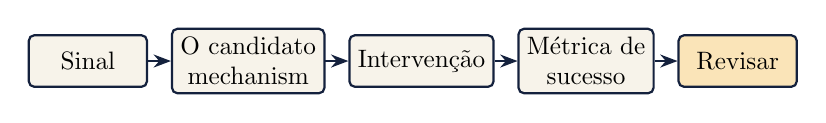
\begin{tikzpicture}[node distance=0.32cm,scale=0.91,transform shape]
    \node[activity] (signal) {Sinal};
    \node[activity,right=of signal] (cause) {O candidato\\mechanism};
    \node[activity,right=of cause] (change) {Intervenção};
    \node[activity,right=of change] (metric) {Métrica de\\sucesso};
    \node[activity,right=of metric,fill=Gold!35] (review) {Revisar};
    \draw[flow] (signal)--(cause);
    \draw[flow] (cause)--(change);
    \draw[flow] (change)--(metric);
    \draw[flow] (metric)--(review);
  \end{tikzpicture}
  \par
  \vspace{0.6cm}
  \keyidea{A mineração de processos apoia a melhoria ao restringir e testar explicações. Ela não estabelece causalidade por si só.}
\end{frame}

% ===========================================================================
% Unidade 10
% ===========================================================================
\lecture{Análise Organizacional e Multidimensional}{10}
\section{Análise organizacional}
\unitdivider{10}{Análise Organizacional e Multidimensional}
  {Processos são redes de coordenação, não apenas sequências de atividades.}

\begin{frame}{Uma rede de transferência de trabalho}
  \centering
  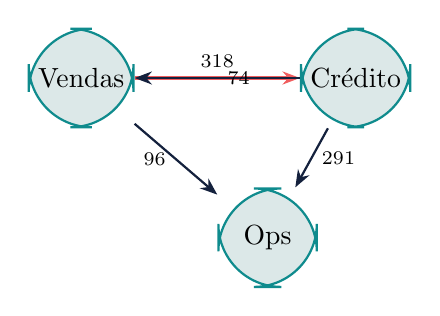
\begin{tikzpicture}[node distance=1.0cm and 2.1cm]
    \node[object,minimum size=1.25cm,rounded corners=8mm] (sales) {Vendas};
    \node[object,right=of sales,minimum size=1.25cm,rounded corners=8mm] (credit) {Crédito};
    \node[object,below right=0.75cm and 1.05cm of sales,minimum size=1.25cm,rounded corners=8mm] (ops) {Ops};
    \draw[accentflow,bend left=12] (sales)--node[above,font=\scriptsize]{318}(credit);
    \draw[flow,bend left=12] (credit)--node[right,font=\scriptsize]{74}(sales);
    \draw[flow] (credit)--node[right,font=\scriptsize]{291}(ops);
    \draw[flow] (sales)--node[left,font=\scriptsize]{96}(ops);
  \end{tikzpicture}
  \vspace{0.45cm}
  A análise de redes pode revelar:
  \begin{itemize}
    \item Transferências frequentes e ciclos de coordenação
    \item Papéis centrais ou sobrecarregados
    \item Questões de segregação de funções
    \item Diferenças entre a colaboração formal e a real
  \end{itemize}
\end{frame}

\begin{frame}{Combine perspectivas}
  \begin{columns}[T,onlytextwidth]
    \column{0.22\textwidth}
      \begin{block}{Fluxo de controle}
        Qual caminho?
      \end{block}
    \column{0.22\textwidth}
      \begin{block}{tempo}
        Quanto tempo?
      \end{block}
    \column{0.22\textwidth}
      \begin{block}{Organização}
        Quem coordenou?
      \end{block}
    \column{0.22\textwidth}
      \begin{block}{dados}
        Sob quais condições?
      \end{block}
  \end{columns}
  \vspace{0.55cm}
  \begin{block}{Exemplo de síntese}
    Os ciclos de esclarecimento são mais lentos quando os casos passam das vendas do parceiro para as operações centrais, especialmente em produtos personalizados com dimensões ausentes.
  \end{block}
\end{frame}

\begin{frame}{Do log de eventos às linhas para aprendizado de máquina}
  \centering
  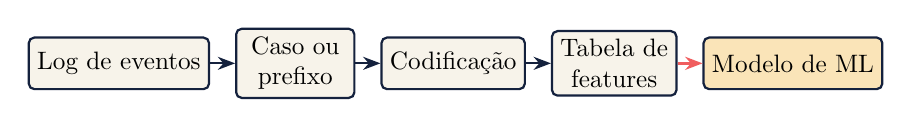
\begin{tikzpicture}[node distance=0.35cm,scale=0.91,transform shape]
    \node[activity] (log) {Log de eventos};
    \node[activity,right=of log] (unit) {Caso ou\\prefixo};
    \node[activity,right=of unit] (encode) {Codificação};
    \node[activity,right=of encode] (features) {Tabela de\\features};
    \node[activity,right=of features,fill=Gold!35] (ml) {Modelo de ML};
    \draw[flow] (log)--(unit);
    \draw[flow] (unit)--(encode);
    \draw[flow] (encode)--(features);
    \draw[accentflow] (features)--(ml);
  \end{tikzpicture}
  \vspace{0.6cm}
  \begin{columns}[T,onlytextwidth]
    \column{0.47\textwidth}
      \textbf{Linha no nível do caso}\\Um caso concluído, geralmente para análise retrospectiva do resultado.
    \column{0.47\textwidth}
      \textbf{Linha no nível do prefixo}\\Um caso observado até um ponto de predição, usado para monitoramento online.
  \end{columns}
  \vspace{0.35cm}
  \keyidea{Defina o corte de observação antes de calcular qualquer feature ou rótulo.}
\end{frame}

\begin{frame}{Estratégias de codificação}
  \scriptsize
  \begin{tabular}{@{}
    >{\raggedright\arraybackslash}p{0.18\textwidth}
    >{\raggedright\arraybackslash}p{0.26\textwidth}
    >{\raggedright\arraybackslash}p{0.25\textwidth}
    >{\raggedright\arraybackslash}p{0.215\textwidth}@{}}
    \toprule
    Codificação & Representação & Ponto forte & Risco principal\\
    \midrule
    Agregação & Contagens, durações, último valor & Baseline simples e sólido & Perde a ordem\\
    Baseada em índice & Atividade/atributo por posição & Preserva a ordem inicial & Tabelas largas e esparsas\\
    Sequência & Tokens ou embeddings aprendidos & Captura ordem e contexto & Demanda dados e computação\\
    Processo-aware & Variante, estado, movimentos de alinhamento & Usa a estrutura do domínio & Viés dependente do modelo\\
    Graph & Features do DFG/grafo de objetos & Captura relações & Validação complexa\\
    Centrada em objetos & Features por tipo de objeto & Evita flattening prematuro & As escolhas de agregação permanecem\\
    \bottomrule
  \end{tabular}
  \vspace{0.45cm}
  \promptbox{Comece com um baseline de agregação. Adicione uma codificação mais rica somente quando ela melhorar a utilidade na validação o bastante para justificar a complexidade.}
\end{frame}

\begin{frame}{A proveniência das features faz parte do modelo}
  Para cada feature, registre:
  \begin{itemize}
    \item Evento de origem ou atributo do objeto
    \item Regra de agregação e de valores ausentes
    \item Primeiro momento em que a feature está disponível
    \item População de casos/objetos à qual se aplica
    \item Parâmetros de pré-processamento ajustados e período de treinamento
  \end{itemize}
  \vspace{0.35cm}
  \begin{block}{Exemplos sensíveis ao processo}
    Contagem de retrabalho, tempo decorrido, atividade atual, prefixo da variante, custo de alinhamento, estado do modelo, número de transferências, objetos abertos e carga de trabalho na chegada.
  \end{block}
\end{frame}

\begin{frame}{Análise responsável de recursos}
  \begin{itemize}
    \item Analise papéis ou equipes antes de indivíduos, quando possível
    \item Verifique carga de trabalho, complexidade dos casos e cobertura dos dados
    \item Evite ranquear pessoas com métricas de processo não validadas
    \item Distinga restrições do processo de desempenho individual
    \item Aplique controle de acesso, minimização e limitação de finalidade
  \end{itemize}
  \vspace{0.45cm}
  \keyidea{Dados de eventos refletem o sistema que atribui o trabalho. Raramente são uma medida isolada justa da contribuição individual.}
\end{frame}

\begin{frame}{Correlação é uma pista, não uma causa}
  Uma equipe pode parecer mais lenta porque recebe:
  \begin{itemize}
    \item Casos mais complexos
    \item Casos já atrasados em etapas anteriores
    \item Trabalho com dados de menor qualidade
    \item Casos que exigem controles adicionais
  \end{itemize}
  \vspace{0.35cm}
  \promptbox{Quais dados adicionais ou desenho de estudo ajudariam a distinguir o efeito da equipe das diferenças no perfil dos casos?}
\end{frame}

% ===========================================================================
% Unidade 11
% ===========================================================================
\lecture{Mineração de Processos Centrada em Objetos}{11}
\section{Mineração centrada em objetos}
\unitdivider{11}{Mineração de Processos Centrada em Objetos}
  {Alguns processos não possuem um único identificador natural de caso.}

\begin{frame}{O problema do flattening}
  \begin{columns}[T,onlytextwidth]
    \column{0.46\textwidth}
      \textbf{Um pedido pode conter}
      \begin{itemize}
        \item Vários itens
        \item Várias entregas
        \item Várias faturas
        \item Um ou mais pagamentos
      \end{itemize}
    \column{0.48\textwidth}
      \begin{block}{Caso forçado por pedido}
        Eventos no nível do item podem ser duplicados no trace achatado.
      \end{block}
      \begin{block}{Caso forçado por item}
        Eventos compartilhados de fatura e entrega podem ser duplicados.
      \end{block}
  \end{columns}
  \vspace{0.4cm}
  Isso cria \textbf{convergência} e \textbf{divergência}: frequências enganosas e relações comportamentais aparentes.
\end{frame}

\begin{frame}{Dados de eventos centrados em objetos}
  \centering
  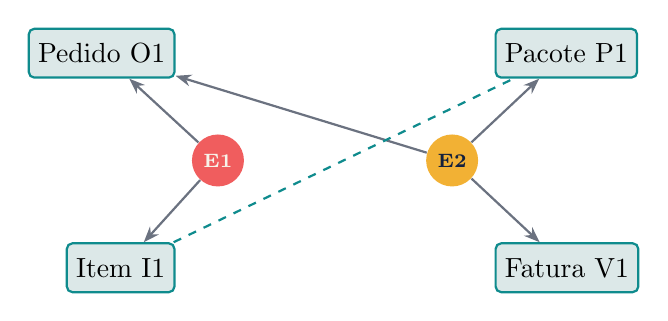
\begin{tikzpicture}[node distance=0.8cm and 1.3cm]
    \node[event] (e1) {E1};
    \node[event,right=2.3cm of e1,fill=Gold,text=Ink] (e2) {E2};
    \node[object,above left=0.8cm and 0.3cm of e1] (order) {Pedido O1};
    \node[object,below left=0.8cm and 0.3cm of e1] (item) {Item I1};
    \node[object,above right=0.8cm and 0.3cm of e2] (pack) {Pacote P1};
    \node[object,below right=0.8cm and 0.3cm of e2] (invoice) {Fatura V1};
    \draw[softflow] (e1)--(order);
    \draw[softflow] (e1)--(item);
    \draw[softflow] (e2)--(order);
    \draw[softflow] (e2)--(pack);
    \draw[softflow] (e2)--(invoice);
    \draw[Teal,thick,dashed] (item)--(pack);
  \end{tikzpicture}
  \vspace{0.55cm}
  OCEL 2.0 representa:
  \begin{itemize}
    \item Eventos ligados a um ou mais objetos tipados
    \item Relações entre objetos
    \item Relações qualificadas e atributos de objetos que mudam
  \end{itemize}
\end{frame}

\begin{frame}{Centrado em casos ou em objetos?}
  \small
  \begin{tabular}{@{}p{0.34\textwidth}p{0.28\textwidth}p{0.28\textwidth}@{}}
    \toprule
    Situação & Caso-centric & Centrada em objetos\\
    \midrule
    Uma instância de negócio estável & Muito adequada & Frequentemente desnecessária\\
    Várias entidades interagindo & Distorce & Muito adequada\\
    KPI estabelecido por caso & Direta & Exige escolhas de agregação\\
    Ferramentas familiares & Maduras & Emergentes\\
    Perguntas sobre relações & Limitada & Nativa\\
    \bottomrule
  \end{tabular}
  \vspace{0.5cm}
  \keyidea{A análise centrada em objetos não elimina escolhas de modelagem. Ela explicita as relações para tornar essas escolhas visíveis.}
\end{frame}

\begin{frame}{Features centradas em objetos sem flattening prematuro}
  \begin{columns}[T,onlytextwidth]
    \column{0.47\textwidth}
      \textbf{Por tipo de objeto}
      \begin{itemize}
        \item Contagens e estados do ciclo de vida
        \item Resumos de idade e tempo decorrido
        \item Objetos relacionados concluídos e abertos
        \item Cardinalidades das relações
      \end{itemize}
    \column{0.47\textwidth}
      \textbf{No momento da predição}
      \begin{itemize}
        \item Congele o grafo de objetos no corte
        \item Agregue somente objetos visíveis
        \item Preserve identificadores para divisões agrupadas
        \item Teste a sensibilidade às regras de agregação
      \end{itemize}
  \end{columns}
  \vspace{0.45cm}
  \keyidea{Faça o flattening tarde e explicitamente. O objeto-alvo e o momento da predição devem determinar quais relações se tornam features.}
\end{frame}

\begin{frame}[fragile]{Inspecione um OCEL com PM4Py}
\begin{lstlisting}[style=python]
import pm4py

ocel = pm4py.read_ocel2_json("order_management.jsonocel")

print(ocel.events.head())
print(ocel.objects.head())
print(ocel.relations.head())

ocdfg = pm4py.discover_ocdfg(ocel)
pm4py.save_vis_ocdfg(ocdfg, "object_centric.svg")
\end{lstlisting}
  \vspace{0.15cm}
  \textbf{Comparação do laboratório:} faça o flattening dos mesmos dados por pedido e por item. Quais frequências ou caminhos se tornam enganosos?
\end{frame}

% ===========================================================================
% Unidade 12
% ===========================================================================
\lecture{Projetos e Comunicação em Mineração de Processos}{12}
\section{Projetos e comunicação}
\unitdivider{12}{Projetos e Comunicação}
  {Um projeto de mineração de processos tem sucesso quando a evidência muda uma decisão.}

\begin{frame}{O ciclo de vida do projeto}
  \centering
  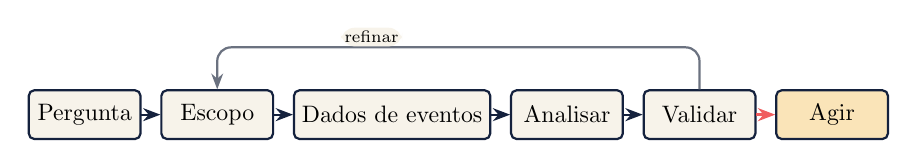
\begin{tikzpicture}[node distance=0.28cm,scale=0.86,transform shape]
    \node[activity] (q) {Pergunta};
    \node[activity,right=of q] (scope) {Escopo};
    \node[activity,right=of scope] (data) {Dados de eventos};
    \node[activity,right=of data] (analyse) {Analisar};
    \node[activity,right=of analyse] (validate) {Validar};
    \node[activity,right=of validate,fill=Gold!35] (act) {Agir};
    \draw[flow] (q)--(scope);
    \draw[flow] (scope)--(data);
    \draw[flow] (data)--(analyse);
    \draw[flow] (analyse)--(validate);
    \draw[accentflow] (validate)--(act);
    \draw[softflow,rounded corners=5pt]
      (validate.north) -- ++(0,0.62)
      -| node[pos=0.34,above,font=\scriptsize,fill=Paper,inner sep=1.5pt]
        {refinar}
      (scope.north);
  \end{tikzpicture}
  \par
  \vspace{0.6cm}
  O ciclo de vida é iterativo. A validação do domínio pode alterar o mapeamento de eventos, a noção de caso, o modelo, a métrica ou até a pergunta original.
\end{frame}

\begin{frame}[shrink=6]{Tarefas de monitoramento preditivo de processos}
  \small
  \begin{tabular}{@{}
    >{\raggedright\arraybackslash}p{0.22\textwidth}
    >{\raggedright\arraybackslash}p{0.24\textwidth}
    >{\raggedright\arraybackslash}p{0.25\textwidth}
    >{\raggedright\arraybackslash}p{0.195\textwidth}@{}}
    \toprule
    Pergunta & Formulação de ML & Exemplo de alvo & Baseline útil\\
    \midrule
    O que acontece a seguir? & Classificação & Próxima atividade & Transição mais frequente\\
    Quanto tempo resta? & Regressão/sobrevivência & Tempo restante & Mediana por estado atual\\
    Como terminará? & Classificação & Atraso / rejeição & Modelo pela taxa-base\\
    Isto é incomum? & Detecção de anomalias & Prefixo desviante & Score de conformidade\\
    \bottomrule
  \end{tabular}
  \vspace{0.45cm}
  \keyidea{A predição deve corresponder a uma decisão operacional e a um momento em que alguém ainda possa agir.}
\end{frame}

\begin{frame}{Prefixos, rótulos e pontos de predição}
  \centering
  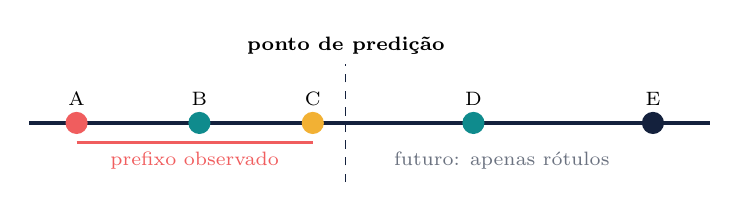
\begin{tikzpicture}[x=1.2cm,y=1cm]
    \draw[very thick,Ink] (0,0)--(7.2,0);
    \foreach \x/\lab/\col in {
      0.5/A/Coral,1.8/B/Teal,3.0/C/Gold,4.7/D/Teal,6.6/E/Ink}
      {
        \fill[\col] (\x,0) circle (4pt);
        \node[above,font=\scriptsize] at (\x,0.10) {\lab};
      }
    \draw[very thick,Coral] (0.5,-0.25)--(3.0,-0.25);
    \draw[dashed,Ink] (3.35,-0.75)--(3.35,0.75);
    \node[below,text=Coral,font=\scriptsize] at (1.75,-0.25)
      {prefixo observado};
    \node[above,font=\scriptsize\bfseries] at (3.35,0.75)
      {ponto de predição};
    \node[below,text=SoftGray,font=\scriptsize] at (5.0,-0.25)
      {futuro: apenas rótulos};
  \end{tikzpicture}
  \vspace{0.55cm}
  \begin{columns}[T,onlytextwidth]
    \column{0.47\textwidth}
      \textbf{Defina}
      \begin{itemize}
        \item Regra e corte do prefixo
        \item Frequência de predição
        \item Horizonte do rótulo
      \end{itemize}
    \column{0.47\textwidth}
      \textbf{Evite}
      \begin{itemize}
        \item Features calculadas após o corte
        \item Rótulos indisponíveis na operação
        \item Prefixos duplicados entre divisões
      \end{itemize}
  \end{columns}
\end{frame}

\begin{frame}{Separe por tempo e agrupe por caso}
  \centering
  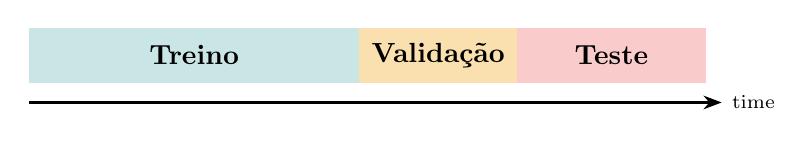
\begin{tikzpicture}[x=1cm,y=1cm]
    \fill[Teal!22] (0,0) rectangle (4.2,0.7);
    \fill[Gold!40] (4.2,0) rectangle (6.2,0.7);
    \fill[Coral!32] (6.2,0) rectangle (8.6,0.7);
    \node at (2.1,0.35) {\textbf{Treino}};
    \node at (5.2,0.35) {\textbf{Validação}};
    \node at (7.4,0.35) {\textbf{Teste}};
    \draw[-{Stealth},thick] (0,-0.25)--(8.8,-0.25)
      node[right,font=\scriptsize]{time};
  \end{tikzpicture}
  \vspace{0.45cm}
  \begin{itemize}
    \item Atribua cada caso e todos os seus prefixos a exatamente uma divisão.
    \item Ajuste codificadores, imputadores, escalonadores e vocabulários apenas nos dados de treino.
    \item Prefira avaliação temporal quando o modelo implantado prevê casos futuros.
    \item Mantenha clientes, pedidos ou objetos relacionados juntos quando houver dependência.
    \item Reserve o período de teste para uma estimativa final após a seleção.
  \end{itemize}
\end{frame}

\begin{frame}{Caminhos comuns de vazamento}
  \begin{columns}[T,onlytextwidth]
    \column{0.47\textwidth}
      \textbf{Vazamento do futuro}
      \begin{itemize}
        \item Atributos finais do caso em um prefixo
        \item Número total de eventos ou duração final
        \item Recurso ou status posterior ao resultado
      \end{itemize}
      \textbf{Vazamento entre divisões}
      \begin{itemize}
        \item Prefixos de um caso em várias divisões
        \item Divisão aleatória no nível dos eventos
      \end{itemize}
    \column{0.47\textwidth}
      \textbf{Vazamento no pré-processamento}
      \begin{itemize}
        \item Normalização ou imputação global
        \item Variantes construídas com todos os períodos
        \item Modelo de descoberta ajustado nos casos de teste
      \end{itemize}
      \textbf{Vazamento operacional}
      \begin{itemize}
        \item Feature indisponível no momento da pontuação
        \item Definição do rótulo muda após a implantação
      \end{itemize}
  \end{columns}
\end{frame}

\begin{frame}{Avalie além da acurácia preditiva}
  \begin{columns}[T,onlytextwidth]
    \column{0.22\textwidth}
      \begin{block}{Discriminação}
        AUC, PR-AUC, MAE, concordance
      \end{block}
    \column{0.22\textwidth}
      \begin{block}{Calibração}
        Confiabilidade, Brier score, cobertura de intervalos
      \end{block}
    \column{0.22\textwidth}
      \begin{block}{Antecedência}
        Antecedência, estabilidade entre prefixos
      \end{block}
    \column{0.22\textwidth}
      \begin{block}{Utilidade}
        Custo, carga de trabalho, atraso evitado, valor da decisão
      \end{block}
  \end{columns}
  \vspace{0.5cm}
  Monitore também:
  \begin{itemize}
    \item Desempenho por coorte e estado do processo
    \item Drift de features, rótulos e processo
    \item Volume de alertas, carga de falsos alarmes e capacidade de intervenção
  \end{itemize}
\end{frame}

\begin{frame}{Padrões de integração: mineração de processos + ML}
  \small
  \begin{columns}[T,onlytextwidth]
    \column{0.47\textwidth}
      \begin{block}{A mineração de processos informa o ML}
        Variantes, estado do modelo, alinhamentos, conformidade, retrabalho e transferências tornam-se features ou coortes.
      \end{block}
      \begin{block}{O ML informa a análise de processos}
        Predições identificam prefixos de risco e revelam onde os erros se concentram no processo.
      \end{block}
    \column{0.47\textwidth}
      \centering
      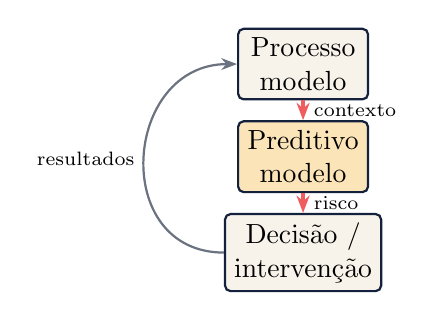
\begin{tikzpicture}[node distance=0.25cm]
        \node[activity] (pm) {Processo\\modelo};
        \node[activity,below=of pm,fill=Gold!35] (ml) {Preditivo\\modelo};
        \node[activity,below=of ml] (action) {Decisão /\\intervenção};
        \draw[accentflow] (pm)--node[right,font=\scriptsize]{contexto}(ml);
        \draw[accentflow] (ml)--node[right,font=\scriptsize]{risco}(action);
        \draw[softflow] (action.west)
          to[out=180,in=180,looseness=1.55]
          node[left,font=\scriptsize]{resultados}(pm.west);
      \end{tikzpicture}
  \end{columns}
  \vspace{0.1cm}
  \keyidea{Versione e monitore o mapeamento de eventos, o modelo de processo, a codificação e o modelo preditivo como um único sistema analítico.}
\end{frame}

\begin{frame}{Uma cadeia de evidências para cada achado}
  \begin{enumerate}
    \item \textbf{Pergunta}: qual decisão está em jogo?
    \item \textbf{Observação}: qual padrão foi medido?
    \item \textbf{Interpretação}: qual mecanismo pode explicá-lo?
    \item \textbf{Validação}: o que especialistas do domínio ou outros dados confirmaram?
    \item \textbf{Ação}: qual mudança deve ser testada?
    \item \textbf{Métrica}: como saberemos se funcionou?
  \end{enumerate}
  \vspace{0.35cm}
  \keyidea{Separe observação de interpretação. Isso torna a análise mais fácil de questionar, melhorar e confiar.}
\end{frame}

\begin{frame}{Comunique bem um achado}
  \begin{columns}[T,onlytextwidth]
    \column{0.46\textwidth}
      \textbf{Comece por}
      \begin{itemize}
        \item Consequência operacional
        \item Magnitude e população afetada
        \item Evidência visual concisa
        \item Próxima ação recomendada
      \end{itemize}
    \column{0.46\textwidth}
      \textbf{Sempre inclua}
      \begin{itemize}
        \item Escopo dos dados
        \item Premissas principais
        \item Incerteza
        \item Alternativas importantes
      \end{itemize}
  \end{columns}
  \vspace{0.45cm}
  \begin{block}{Padrão de título}
    \alert{O que acontece} + \alert{onde} + \alert{impacto}: ``Ciclos de esclarecimento adicionam 4,1 dias aos pedidos personalizados do canal parceiro.''
  \end{block}
\end{frame}

\begin{frame}{Checklist de reprodutibilidade}
  \begin{columns}[T,onlytextwidth]
    \column{0.47\textwidth}
      \begin{itemize}
        \item Código versionado de extração e transformação
        \item Dicionário de dados e semântica dos eventos
        \item Parâmetros fixos e versões dos pacotes
        \item Figuras e tabelas determinísticas
      \end{itemize}
    \column{0.47\textwidth}
      \begin{itemize}
        \item Exclusões e filtros documentados
        \item Artefatos de modelo armazenados
        \item Log de decisões e validações
        \item Estratégia de compartilhamento sensível à privacidade
      \end{itemize}
  \end{columns}
  \vspace{0.5cm}
  \promptbox{Outro analista conseguiria reproduzir seu achado central sem perguntar onde você clicou?}
\end{frame}

\begin{frame}[shrink=8]{Oportunidades de pesquisa}
  \small
  \begin{columns}[T,onlytextwidth]
    \column{0.47\textwidth}
      \textbf{Dados de eventos mais ricos}
      \begin{itemize}
        \item Logs de eventos multimodais
        \item Abstração automatizada de eventos
        \item Eventos centrados em objetos, em streaming e incertos
      \end{itemize}
    \column{0.47\textwidth}
      \textbf{Análises mais ricas}
      \begin{itemize}
        \item Aprendizado de representações multimodais
        \item Mineração causal de processos
        \item Monitoramento prescritivo
        \item Análises com preservação de privacidade
      \end{itemize}
  \end{columns}
  \vspace{0.15cm}
  \begin{block}{Logs de eventos multimodais}
    Alinhe eventos estruturados com payloads como texto livre, documentos, imagens, áudio e fluxos de sensores, preservando tempo, proveniência e regras de acesso.
  \end{block}
  \vspace{0.05cm}
  \keyidea{Cada modalidade deve acrescentar evidência de processo válida, oportuna e governável.}
\end{frame}

% ===========================================================================
% Projeto final e close
% ===========================================================================
\lecture{Projeto final e encerramento do curso}{13}
\section{Projeto final}

\begin{frame}{Projeto final: estudo de processo ponta a ponta}
  \begin{columns}[T,onlytextwidth]
    \column{0.48\textwidth}
      \textbf{Análise obrigatória}
      \begin{itemize}
        \item Escopo e perguntas analíticas
        \item Semântica dos eventos e relatório de qualidade
        \item Representação, flattening e codificação
        \item Exploração, desempenho e descoberta
        \item Vetor de qualidade e comparação pela fronteira de Pareto
        \item Análise de conformidade ou desvios
      \end{itemize}
    \column{0.48\textwidth}
      \textbf{Argumentação obrigatória}
      \begin{itemize}
        \item Um achado validado
        \item Baseline preditivo quando relevante
        \item Divisão e avaliação sem vazamento
        \item Uma hipótese de melhoria
        \item Limitações éticas e analíticas
        \item Código e artefatos reproduzíveis
        \item Apresentação orientada aos stakeholders
      \end{itemize}
  \end{columns}
\end{frame}

\begin{frame}{Avaliação do projeto final}
  \small
  \begin{tabular}{@{}p{0.30\textwidth}p{0.58\textwidth}@{}}
    \toprule
    Dimensão & Evidência de um trabalho sólido\\
    \midrule
    Pergunta e escopo & Decisão específica, noção de caso coerente e limites explícitos\\
    Representação & Semântica validada, flattening e codificação justificados\\
    Qualidade do modelo & Vetores completos de métricas, análise de Pareto e regra de seleção estável\\
    Predição & Divisão sem vazamento, erros calibrados e baseline operacional\\
    Interpretação & Achados distinguem evidência de explicação\\
    Reprodutibilidade & A análise executa das entradas documentadas até as saídas\\
    Comunicação & Consequência, incerteza e próxima ação estão claras\\
    \bottomrule
  \end{tabular}
\end{frame}

\begin{frame}{A disciplina do analista}
  \Large
  \begin{enumerate}
    \item Questione a semântica dos eventos.
    \item Torne explícitas as escolhas de representação.
    \item compare vetores de qualidade, não uma única pontuação.
    \item Previna vazamento antes do treinamento.
    \item Transforme achados e predições em ações testáveis.
  \end{enumerate}
  \vspace{0.35cm}
  \keyidea{A habilidade mais importante em mineração de processos é saber o que os dados permitem afirmar.}
\end{frame}

\begin{frame}[plain]
  \begin{tikzpicture}[remember picture,overlay]
    \fill[DeepInk] (current page.south west) rectangle (current page.north east);
    \fill[Coral] (current page.south west) rectangle
      ([yshift=0.13\paperheight]current page.south east);
    \node[text=Paper,font=\fontsize{31}{34}\selectfont\bfseries]
      at ([yshift=0.55cm]current page.center) {Perguntas tornam-se evidências.};
    \node[text=Mist,font=\Large]
      at ([yshift=-0.75cm]current page.center) {Evidências tornam-se melhores decisões de processo.};
    \node[text=Paper,font=\small]
      at ([yshift=0.065\paperheight]current page.south) {\coursename\quad|\quad\instructor};
  \end{tikzpicture}
\end{frame}

\end{document}
